\documentclass[11pt,]{article}

\linespread{1.5}

\usepackage[switch]{lineno}
\let\oldequation\equation
\let\oldendequation\endequation

\renewenvironment{equation}
  {\linenomathNonumbers\oldequation}
  {\oldendequation\endlinenomath}

\usepackage{titlesec}

\setcounter{secnumdepth}{4}

\titleformat{\paragraph}
{\normalfont\normalsize\bfseries}{\theparagraph}{1em}{}
\titlespacing*{\paragraph}
{0pt}{3.25ex plus 1ex minus .2ex}{1.5ex plus .2ex}
\usepackage{a4wide}

\usepackage{graphicx}
\DeclareGraphicsExtensions{.pdf}

\usepackage[labelformat=empty, position=top]{subcaption}
\usepackage[export]{adjustbox}
\usepackage{authblk}
\usepackage{amsmath}
\usepackage{amsfonts}
\usepackage[utf8]{inputenc}
\usepackage{hyperref}

\usepackage{siunitx}
\sisetup{range-units=single,
        separate-uncertainty = true,
        multi-part-units = single,
        per-mode=symbol,
        inter-unit-product = \ensuremath { { } \cdot { } }
        }

\usepackage{tabularx}
\usepackage{booktabs}
\usepackage{color}

\newcommand{\supplementarysection}{%
  \setcounter{figure}{0}% Reset figure counter
  \setcounter{table}{0}
  \let\oldthefigure\thefigure% Capture figure numbering scheme
  \let\oldthetable\thetable
  \renewcommand{\thefigure}{S\oldthefigure}% Prefix figure number with S
  \renewcommand{\thetable}{S\oldthetable}
  \section{Supplementary material}% Set supplementary section
  \let\oldsection\section% Copy \section into \oldsection
  \renewcommand{\section}{% Update \section
    \let\thefigure\oldthefigure% Copy \thefigure into \oldthefigure
    \let\section\oldsection% Restore original \section
    \oldsection% Call original \section
  }
}

\graphicspath{{./imgs-pdf/}}
\usepackage[numbers, sort]{natbib}
\bibliographystyle{abbrvnat}

\title{Linking Structure and Function: Image-Based Virtual Populations of the Retinal Vasculature}
\date{\today}
% \author{R\'emi J. Hernandez\\ Department of Cardiovascular and Metabolic Medicine, University of Liverpool
%   \and Yalin Zheng\\ Department of Eye and Vision Science, University of Liverpool
%   \and Savita Madhusudhan\\ Liverpool Ophthalmic Reading Centre, St Paul's Eye Unit, Royal Liverpool University Hospitals NHS Trust
%   \and Wahbi K. El-Bouri\\ Department of Cardiovascular and Metabolic Medicine, University of Liverpool}

\author[1,2]{R\'{e}mi Hernandez\footnote{E-mail address: remi.hernandez@liverpool.ac.uk (R\'{e}mi Hernandez)}}
\author[3,4]{Savita Madhusudhan}
\author[3,4]{Yalin Zheng}
\author[1,2]{Wahbi K. El-Bouri\footnote{E-mail address: w.el-bouri@liverpool.ac.uk (Wahbi K. El-Bouri)}}

\affil[1]{Liverpool Centre for Cardiovascular Science, University of Liverpool and Liverpool Heart \& Chest Hospital Liverpool, UK}                                                                               
\affil[2]{Department of Cardiovascular and Metabolic Medicine, Institute of Life Course and Medical Sciences, University of Liverpool, UK}
\affil[3]{St Paul's Eye Unit, Liverpool University Hospitals NHS Foundation Trust, Liverpool, UK}
\affil[4]{Department of Eye and Vision Science, Institute of Life Course and Medical Sciences, University of Liverpool, UK}

\providecommand{\keywords}[1]{\textbf{\textit{Keywords---}} #1}

\begin{document}

\maketitle

\begin{abstract}
  \textbf{Purpose:} We developed a novel framework to generate virtual vasculature of the macula, from the central retinal vessels down to the macular capillaries, alongside a haemodynamics model which tests the associations between vascular morphology as delineated by optical coherence tomography angiography (OCTA) and retinal perfusion.

  \textbf{Methods:} The method to generate the vasculature is based on the distribution of few clinical parameters pertaining to the central retinal vessels, constructive constrained optimisation (CCO) and Voronoi diagram.
  Arterial and venous trees are generated in the temporal retina and connected through three layers of capillaries at different depths in the macula.
  Morphology of the virtual vasculatures is compared with OCTA data.
  Associations between total retinal blood flow and macular flow fraction and vascular morphology are derived as Spearman rank coefficients and uncertainty from input parameters is quantified.
  
  \textbf{Results:} A virtual cohort of \SI{200}{} healthy vasculatures were generated.
  Vessel area density (VAD), fractal dimension (FD) and inter-vessel distance were in good agreement with pusblished values.
  Total retinal blood flow was strongly correlated with VAD, vessel diameter index (VDI), FD and vessel calibre index (VCI).
  The macular flow fraction was not correlated with any morphological metrics.

  \textbf{Conclusions:} The proposed framework is able to reproduce vascular networks in the macula that are morphologically and functionally similar to real vasculature.
  The framework provides quantitative insights into how macular perfusion can be affected by changes in vascular morphology delineated on OCTA.
    
\end{abstract}

\begin{keywords}
  % Digital twins, \textit{In-silico} trials,
  Macula, Computational model, Sensitivity analysis, Haemodynamics, Digital twins, \textit{In silico} model
\end{keywords}

%\linenumbers
\section{Introduction}\label{introduction}

The retina is a highly oxygen-dependant, complex band of tissue at the back of the eye which plays a key role in visual function.
It requires close interplay between many different cell types and supporting structures, including a complex vascular system~\cite{Hernandez2023}.
As a result, the retina is sensitive to small changes which may lead to loss of visual functions.
\textit{In silico} modelling has the potential to offer insight into the complex interactions between the retinal environment and the underlying causes of retinal diseases.
In particular virtual populations and \textit{in silico} clinical trials are a promising way to enhance basic research and clinical trials~\cite{Hernandez2023}.
Optical coherence tomography angiography (OCTA) is a non-invasive, new imaging modality that offers three dimensional, high resolution angiograms of the macula, which is the central-most area of the retina.
Several microvascular metrics, such as vessel density and fractal dimension, have been suggested to quantify the quality of the microvasculature on OCTAs~\cite{Chu2016}.
Using those metrics, several microvascular changes have been linked with ageing and diseased retinae\cite{Ma2021,Trinh_2019, Told2023} and also with cerebrovascular changes and cardiovascular diseases~\cite{Pleouras_2021,Graff_2021,LopezCuenca_2022}.
For the latter two, virtual populations have been developed, but similar work is yet to be done for the retinal vasculature or for the linked cerebral-retinal vasculature~\cite{Hernandez2023}.

Such alterations to the retinal and choroidal vasculature are expected to negatively affect the perfusion of the retina.
Ischaemia and hypoxia are likely involved in the pathogenesis of several retinal diseases, in
particular neovascular diseases such as neovascular age-related
macular degeneration, proliferative diabetic retinopathy or retinal
vein occlusion which are characterised by pathological growth of blood
vessels through angiogenesis~\cite{Medina_2016}.
Hypoxia is a known trigger of angiogenesis and targeting ischemia-induced angiogenic pathways might improve treatment outcomes~\cite{UsuiOuchi2020}.

However, owing to the difficulty of experimentally measuring oxygen
levels in the retina, the role of hypoxia in the pathogenesis of
neovascular diseases remains unclear. Furthermore, it also remains unclear
how changes in microvascular metrics computed on OCTAs relate to the
quality of blood perfusion. Computational models of the retina and its
vasculature, combined with mathematical models of haemodynamics and
oxygen transport, can help in linking structure and function.

Retinal haemodynamics and oxygenation have received considerable
attention from the modelling community in recent
years~\cite{Arciero2008,Bernabeu2014,Causin2016,Chiaravalli2022,DoblhoffDier2014,
  Fry2020,Guidoboni2014,Hernandez2023,Takahashi2009,Zhu2019,Yu2019}.
Compartmental models~\cite{Arciero2008,Guidoboni2014,Chiaravalli2022}
or symmetrical branching
networks~\cite{Chiaravalli2022,Takahashi2009,Zhu2019} are used in many
of these models. These approaches are favoured for their simplicity
and adaptability to systems with limited information. However, they
fail to reproduce the heterogeneity of the retinal
vasculature~\cite{Yu2019}. In contrast, models based on vascular
networks reconstructed from imaging data~\cite{Bernabeu2014,Fry2020}
are more faithful to the physiology of the retina, but the
reconstruction of the network is arduous and therefore only a limited
number of eyes can be modelled. Space-filling algorithms are a way to
circumvent these problems by generating heterogeneous networks with
similar characteristics to real
vasculature~\cite{Causin2016,Linninger2013,Talou2021}. For instance,
Causin et al.~\cite{Causin2016} used diffusion-limited aggregation because it creates structures with a fractal dimension similar to that of retinal vasculature.
The class of space-filling algorithms called constrained constructive algorithms
(CCO) is another approach that includes rules and constraints meant to
reproduce the angiogenesis process~\cite{Linninger2013,Talou2021}. It
has been applied to the retinal
vasculature~\cite{Brown2023,LoCastro2020}, but only to create
synthetic data for deep learning applications. Despite the interest of
the research community in retinal haemodynamics, little quantitative
experimental work has been done. As a result, most models are
validated against the same data~\cite{DoblhoffDier2014,Riva1985}.

This paper presents a framework for generating virtual populations of
the microvasculature of the macula, using a few clinical measurements as
inputs. The framework proposed in Section~\ref{sec:methods} includes a
partial representation of the larger arteries and veins of the
temporal retina, branching from the central retinal artery (CRA) and
vein (CRV); a full representation of the macular microvasculature,
with arterioles and venules connected through a capillary bed; and a
haemodynamics model. In Section~\ref{sec:validation}, we add a layer
of validation compared to other retinal haemodynamics models by
comparing the microvascular structure of the model with OCTA
metrics. In Section~\ref{sec:gsaUQ}, global sensitivity analysis
techniques are applied to each aspect of the model to
quantify the uncertainty brought about by the uncertainty in clinical
parameters and model hyper-parameters. Section~\ref{sec:discussion}
contains a discussion of the results, while
Section~\ref{sec:conclusion} summarises the conclusions and future
perspectives.

\section{Methods}\label{sec:methods}

In this section we describe the proposed models.
Section~\ref{sec:structModel} describes the model generating the
retinal vasculature, from the macro to micro scale.
Section~\ref{sec:haemodynamicModel} describes the proposed haemodynamic
model.

\begin{figure}[ht!] \centering
    \centering
  \begin{subfigure}[t]{.02\textwidth}
    \scalebox{1}{\adjustbox{valign=T}{\textbf{A}}}
  \end{subfigure}
  \begin{subfigure}[t]{.6\textwidth}
    \scalebox{1}{\adjustbox{valign=T}{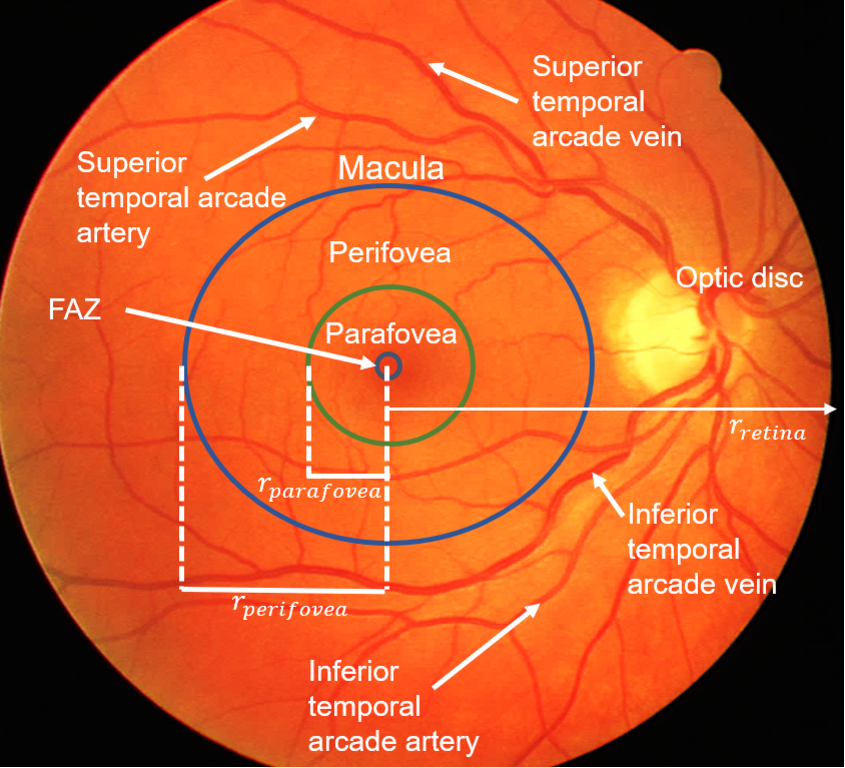
\includegraphics[width=\textwidth, valign=t]{Figure1A.pdf}}}
  \end{subfigure}
%  \hfill
  \\
  \begin{subfigure}[t]{.02\textwidth}
    \scalebox{1}{\adjustbox{valign=T}{\textbf{B}}}
  \end{subfigure}
  \begin{subfigure}[t]{.58\textwidth}
    \scalebox{1}{\adjustbox{valign=T}{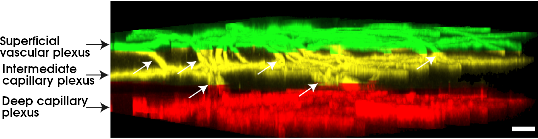
\includegraphics[width=\textwidth, valign=t]{Figure1B.pdf}}}
  \end{subfigure}

  \caption{Architecture of the retina. (\textbf{A}) Landmarks of the retina on a \SI{45}{\degree} field-of-view colour fundus photograph from the DRIVE data-set~\cite{Staal_2004}.
  (\textbf{B}) The three capillary layers of the macula imaged with histology. Image from the work of~\citet{An2020}, available under a CC BY-NC-ND license.}
  \label{fig:1}
\end{figure}

\subsection{Structural model}\label{sec:structModel}

The structural model generates retinal vasculature from the macro
scale (arteries, arterioles, veins and venules) to the micro scale
(capillaries).

Macroscale vasculature is generated on the temporal retina, starting
from the CRA and ending in the CRV.  First, a statistical shape model~\cite{Davies_2008}
of the major temporal arcades was developed using a fundus
photographs data-set.  The remaining superficial temporal vasculature is
partially generated with a constructive constrained optimisation (CCO)
algorithm~\cite{Talou2021}.

Microvasculature is generated in the macula area (see
Figure~\ref{fig:1}) across three vascular layers, namely superficial
vascular plexus (SVP), intermediate(ICP) and deep capillary plexuses
(DCP), arranged as parallel, planar layers at fixed depths \(z\).
In contrast, the macrovasculature is only generated in the SVP.
This is because the ICP and DCP are composed of capillaries in the perifovea and merge with the SVP outside the macula~\cite{An2021}.

\subsubsection{Macrovasculature}

\paragraph{Statistical shape model}

Major temporal arcade vessels were manually segmented from the DRIVE data-set~\cite{Staal_2004}.
The major temporal arcade vessels correspond to the four
vessels (two veins, two arteries) that branch directly from the
central retinal vessels and extend towards the superotemporal and inferotemporal quadrants of 
the retina (see Figure~\ref{fig:1} for an example of the temporal
arcades).  Vessel centreline segmentations, from their branching at
the level of the optic disc to the boundary of the visible retina,
were extracted from 8 colour fundus photographs centred on the fovea.
Images were excluded if the arteries and veins could not be
confidently differentiated or if the eye presented pathologies, as
reported in the data-set.  Segmentation was performed using the
`freehand line' tool in ImageJ 1.48~\cite{Schneider2012}.  The pixel
coordinates for each curve were extracted and translated so that the
fovea is at the origin.  This ensures that the model learns the
distance between the optic disc and the fovea and between the arcades
and the fovea, which may have importance in disease~\cite{Arslan2021}.
For images of right eyes, curves are reflected across the y-axis so that all shapes correspond to left eyes
(i.e., optic disc on the left-hand side of the image).
\\
The extracted curves were then smoothed using B-splines and their
inflection points computed. For a B-spline curve
$\Gamma(t)=\left(x(t),y(t)\right)$ sampled at times $t_i,\ i=1,…,k$,
the inflection points are times $t_i$ where
$\varphi(t)=x^\prime(t)y^{\prime\prime}(t)-x^{\prime\prime}(t)y^\prime(t)$
changes sign, i.e.,
$sign(\varphi(t_{i-1}))-sign(\varphi(t_i))\neq0$. In this work, we
used $k=30$ and $t_i=i k^{-1}$ to compute the inflection
points. Higher sampling rates lead to more inflections points. The
start and end points of the curves along with the inflection points
form the primary training data-set for the statistical shape
model. Because not all segmented curves yield the same amount of
inflection points, we up sample the curves by splitting the longest
vessels in half, repeating as necessary. This results in 4 training
sets, one for each arcade, with varying number of training points
between sets. All shapes in a training set are aligned using the
Kabsch-Umeyama algorithm \cite{Umeyama1991}. Effectively, all shapes are
rotated, translated and scaled as to minimise the least mean-squared
error between the shapes and their (aligned) mean.
\\
For arcade vessel $j$, with $m_j$ points in each shape, a data matrix
$X_j\in\mathbb R^{2m_j,n}$ is assembled by stacking the curves
row-wise. Denoting $(e_{j,i}, \lambda_{j,i})$ the eigenvectors and
associated eigenvalues of the Pearson correlation matrix of $X_j$,
construct $P_j\in\mathbb R^{2m_j,l_j}$ by stacking the $l_j$
eigenvectors with the largest eigenvalues column-wise. The number of
modes of variations $l_j$ may be chosen as to explain $>95\%$ of the
variance in the data. Finally, denoting $\bar x_j$ the mean of all
shapes, one can create a new, unique shape x using $x=\bar x_j + P_jb$
where $b\sim\mathcal N(0,diag(\lambda_{j,i}, i=1,...,l_j))$. The
resulting $m_j$ points are interpolated using centripetal Catmull-Rom splines~\cite{Catmull_1974} before being used in the next steps.
The generated shapes are converted to length units using the rule of thumb for fundus photographs: $\SI{10}{\degree}\approx\SI{5}{\mm}$, where the angle describes the
field of view of the fundus camera. The generated vessels are linked
to the central retinal vein or central retinal artery accordingly and
assume the same radius as the central retinal vessels.
The radius of the central retinal artery (CRA) is given in Table~\ref{tab:parameters} whereas the radius of the
central retinal vein (CRV) is larger by a factor $1.11$~\cite{Goldenberg2013}.

\paragraph{Arterial/venous branching trees}\label{sec:CCO}

From each output of the statistical shape model, a pair of trees, one
arterial and one venous, is generated.

At this stage, trees are structured branching trees using a
space-filling algorithm. The algorithm is a modification of the
constrained constructive optimisation (CCO) algorithm proposed
by~\cite{Talou2021}. With the CCO, trees are grown to minimise the tree’s
total volume while, for each addition of vessel segments,
keeping a constant pressure drop from
inlet to outlet and satisfying several geometrical constraints.

In addition to the original CCO’s constraints, tree growth is
geometrically constrained to prevent vessels from crossing the line
that passes through the optic disc centre and the centre of the fovea,
which separates the superior and inferior halves of the
retina. Additionally, we used a custom probability distribution
(see Table~\ref{tab:parameters}) 
to select the location of new vessel segments to mimic an angiogenic
process biased towards the fovea, while keeping the foveal avascular
zone (FAZ) free of vessels. 
Indeed, the fovea has higher concentration
of cells, and therefore more metabolic needs, compared to the rest of
the retina~\cite{Zouache2022}.
The CCO is applied in three stages, within three circular regions: in
a disk of radius $r_{retina}$, in a annulus with radii $r_{parafovea},
r_{perifovea}$ and finally in a disk of radius $r_{parafovea}$
(see Figure~\ref{fig:1}).

To simulate growth biased towards the fovea while keeping the FAZ free
of vessels, the coordinates of a segment endpoint are given by
$(x,y)=(r\cos\theta, r\sin\theta)$, where $\theta$ follows a uniform
distribution over the interval $[0,2\pi)$ and $r$ follows a lognormal
distribution (see Table~\ref{tab:parameters}). Arterio-venous
networks of the superficial vascular plexus are generated in three
steps: 1) the CCO is applied to create a backbone of larger arterioles
and venules from the arterial and venous arcades. The arterial and
venous backbones are grown separately in the first step. For each
tree, the CCO requires volumetric blood flow at the root (CRA or CRV)
and a pressure drop across the vasculature. Blood flow in the CRA is
computed from its radius and blood flow velocity. From conservation of
mass, blood flow is the same in the CRV.
Ocular perfusion pressure (OPP) refers to the pressure drop between the CRA and CRV, namely:
\begin{equation}
OPP=p_{CRA}-p_{CRV}.\label{eq:OPP}
\end{equation}
Pressure in the CRV is assumed equal to IOP~\cite{Arciero2013,Guidoboni2014,Zheng2010}.
Pressure in the CRA is estimated as two thirds of the mean arterial pressure (MAP)~\cite{Arciero2013,Guidoboni2014,Zheng2010}:
\begin{equation}
p_{CRA}=\frac23MAP\label{eq:pCRA}
\end{equation}
The pressure drop across the vascular trees are set to
$p_{pre-capillary}-p_{CRV}$ for the venous tree and
$p_{CRA}-p_{pre-capillary}$ for the arterial trees. The value of
$p_{pre-capillary}$ is taken from pressure in pre- and post-capillary vessels in
the theoretical model by \citet{Takahashi2009} and reported in
Table~\ref{tab:parameters}.

\paragraph{Microvasculature}\label{sec:microvasculature} At the macro
scale, arterioles and venules generally follow a bifurcating
structure, with parent vessels giving rise to two daughter
branches. The CCO algorithm follows this logic to create vascular
trees.  At the micro scale, however, capillaries tend to form complex
nets, forming loops and anastomoses~\cite{An2020} that are
incompatible with the CCO’s logic.
Therefore, we adopt the methodology proposed by~\citet{Linninger2013} to generate capillary beds connecting
the arterial and venous trees.  In short, a disk the size of the
macula (see Table~\ref{tab:parameters}) is meshed with a Delaunay
triangulation generated from $N_{Seeds}$ randomly sampled points
within the disk.
The centroids of the triangles are used to generate a Voronoi diagram.
In brief, a Voronoi diagram partitions the plane into polygonal regions centred around input points. 
The edges of the polygons form the capillary bed.
In the SVP, capillaries coexist with arterioles and venules, but should not intersect them.
Therefore, capillaries intersecting with arterioles or venules are removed from the capillary bed.
This also creates a capillary-free region which is found surrounding arterioles in the SVP~\cite{An2020}.

In the SVP, a proportion $\alpha$ of arterioles and venules and all terminal vessels within the macula are connected to the nearest capillary. Because of the lack of specific data, $\alpha$ was arbitrarily set to \SI{40}{\percent} in all simulations unless specified otherwise.

Inter-plexi connections remain subject to debate~\cite{An2020,Chiaravalli2022,Campbell2017}.
Since the ICP and DCP are modelled in the macula only, inter-plexi connections are based on the findings by \citet{An2020} in the parafovea.
Specifically, arterioles and venules within the macular area of the SVP bifurcate to the ICP and those branches immediately bifurcate to the DCP.
This corresponds to the most prevalent patterns in the histology study~\cite{An2020}.
From the SVP, \SI{30}{\percent} of the arterioles and venules were selected for bifurcation to the ICP and the bifurcation points were added in the middle of the selected vessels.

All capillaries are initially given the same radius $r_{capillary}$ unless they are connected to an arteriole or venule, in which case their initial radius is twice that of other capillaries.
Diameter transitions at bifurcations are smoothed using the method proposed by \citet{Linninger2013}.
With this method, the diameter of a segment is changed to the average diameter of the segments it is connected to.

The last necessary step for haemodynamics simulation is to give direction to the capillaries create from the Voronoi diagram.
This can be achieve by using the diffusion equation.
Representing the vasculature as a graph, temperatures are assigned to nodes: $1$ for arterial nodes, $0$ for venous nodes and $0.5$ for capillary nodes.
The graph Laplacian of the vasculature is used to update the nodes' temperature.
The temperatures provide an ordering of the capillaries, from hot to cold, that ensures the graph remains acyclic, which is a necessary condition for haemodynamics simulations.

\begin{figure}[ht!]
  \centering
  \begin{subfigure}[t]{.02\textwidth}
    \scalebox{1}{\adjustbox{valign=T}{\textbf{A}}}
  \end{subfigure}
  \begin{subfigure}[t]{.95\textwidth}
    {
      \fontsize{3pt}{4pt}\selectfont% or whatever fontsize you like
      \def\svgwidth{\textwidth}    
      \scalebox{1}{\adjustbox{valign=T}{\input{imgs-pdf/PrettyPicture.pdf_tex}}}
    }
  \end{subfigure}
  % \hfill
  \\
  \begin{subfigure}[t]{.02\textwidth}
    \scalebox{1}{\adjustbox{valign=T}{\textbf{B}}}
  \end{subfigure}
  \begin{subfigure}[t]{.95\textwidth}
    \scalebox{1}{\adjustbox{valign=T}{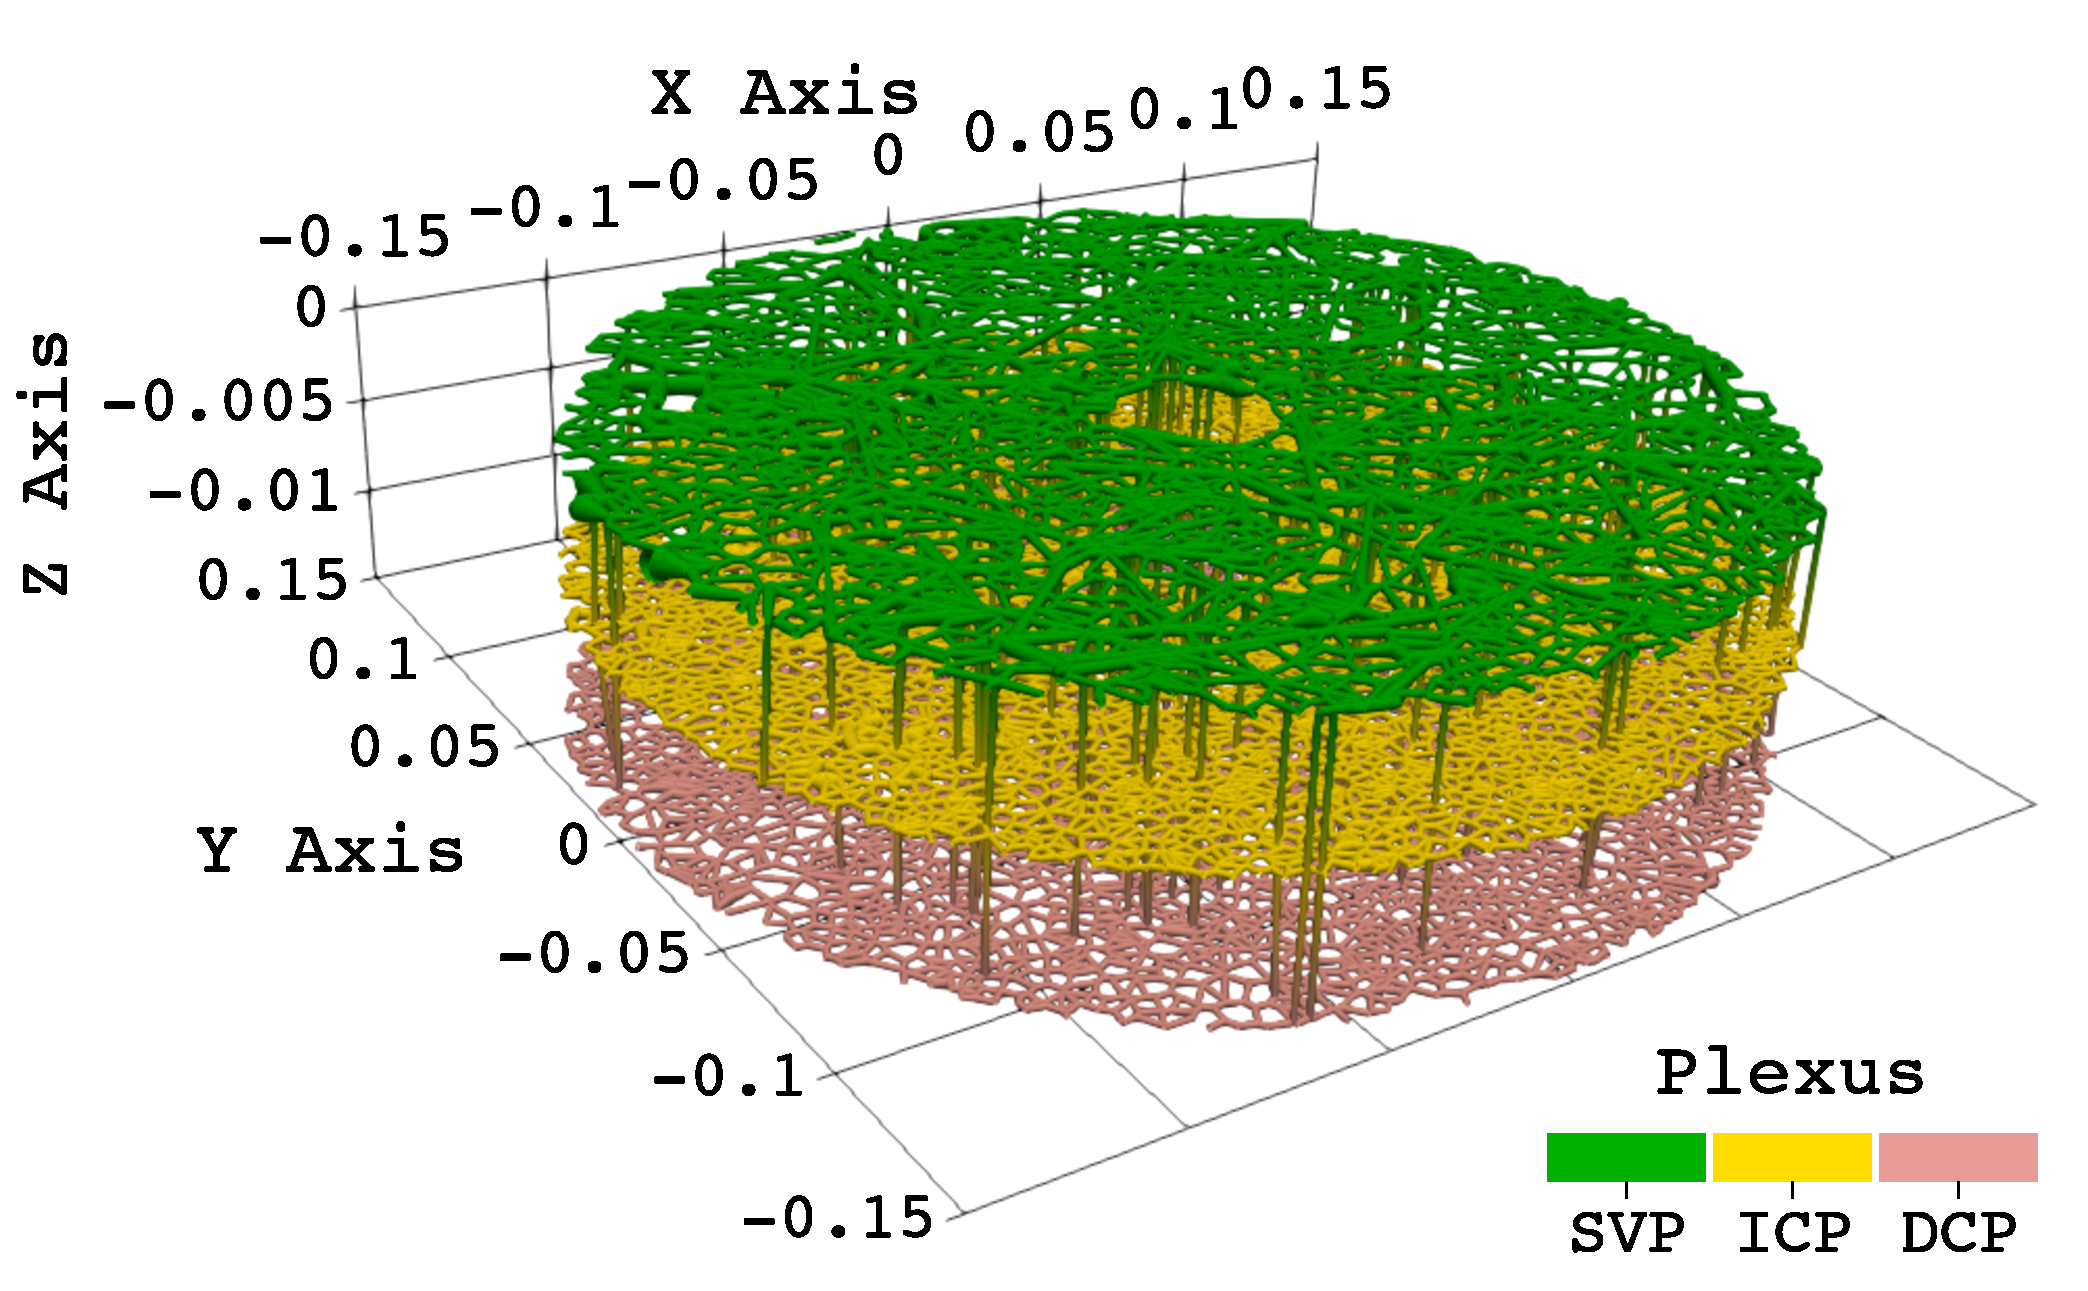
\includegraphics[width=\textwidth, valign=t]{Figure2B.pdf}}}
  \end{subfigure}

  \caption{ % Construction of the microvasculature of the macula. A
    % capillary bed is generated in the superficial vascular plexus as a Voronoi diagram (in blue).
    % Capillaries intersecting arterioles or venules are removed
    % (\textbf A). In (\textbf A), venules are shown in green,
    % arterioles in red and capillaries in blue. Dashed blue lines are
    % capillaries that are removed because intersecting with other
    % vessels. Similar capillary beds are generated for the intermediate
    % and deep capillary plexi, without the need to remove
    % intersections. Capillaries are linked with arterioles and venules
    % to create a complete vascular network (\textbf B).
    (\textbf{A}) The haemodynamics simulations use blood pressure at the CRA and CRV as inputs.
    Outside the macula, terminal arteries are linked to a compartment through an artificial resistance $\mathcal{R}$
    which redistributes the flow to terminal veins through connection with the same resistance $\mathcal{R}$.
    In the macula, capillaries connect arteries to veins across three vascular plexi (\textbf{B}).
    SVP: superficial vascular plexus. ICP: intermediate capillary plexus. DCP: deep capillary plexus.
  }
  \label{fig:fig2}
\end{figure}

\subsection{Haemodynamics model}\label{sec:haemodynamicModel}

Blood is modelled as an incompressible, Newtonian fluid flowing in a
network of connected tubes by the Hagen-Poiseuille equation.
This modelling framework considers the
vasculature as a arrangement of connected, straight tubes across which
pressure drop $\Delta p$, vascular resistance $R$ and volumetric blood
flow $Q$ are related by:
\begin{equation}
  \label{eq:poiseuille}
%  \Delta p=Q\times R
  Q = \frac{\Delta p}{R}.
\end{equation}
Vascular resistance is a function of the tube's radius $r$, length $l$
and the blood viscosity $\mu$ as follows:
\begin{equation}
  \label{eq:resistance}
  R=\frac{8\mu l}{\pi r^4}.  
\end{equation}
Blood is a non-Newtonian fluid and is subject to the
F\r{a}hr\ae us–Lindqvist effect~\cite{Faahraeus1931} in the
microcirculation. 
Non-Newtonian effects are accounted for by a radius-dependent,
empirical, effective viscosity law~\cite{Secomb2013}:
\begin{equation}
  \label{eq:viscosity}
  \mu(r)=1+(\mu_{0.45}-1)\frac{(1-H_D)^C-1}{(1-0.45)^C-1},
\end{equation}
where $\mu_{0.45}$ and $C$ are empirical constants and $H_D$ is the
discharge haematocrit.
Discharge haematocrit is kept constant at \SI{45}{\percent} in this work.

In the macular area, the vasculature is fully connected, with
arterioles connecting to venules through capillaries.
Outside the macula, however, the first stage of the CCO detailed in
Section~\ref{sec:CCO} leaves terminal vessels with no further branches, both on the arterial and venous sides, which need to somehow be linked to the central retinal vessels.
This happens as a result of not generating the full extent of the peripheral vasculature.
To close the vascular network, these terminal vessels need to somehow be linked to the CRA/CRV or haemodynamics in those vessels need to be explicitly given.
In the absence of adequate data on haemodynamics for those vessels, we chose to instead link the terminal vessels through a compartment.
All terminal arteries outflow into the compartment through artificial vessels with a resistance $\mathcal R$.
All terminal veins drain the vascular compartment through artificial vessels with the same resistance. 
The macula has twice the density of cells compared to the rest of the retina~\cite{Zouache2022}.
Assuming that regions of higher cell density require similarly higher blood flow, it can be estimated that the macula requires \SIrange{15}{30}{\percent} of the total retinal blood flow.
The baseline value of parameter $\mathcal R$ was selected such that the blood flow rates into the macula are within this range for the baseline simulations.

\begin{table}
  \def\tabularxcolumn#1{m{#1}}
  \newcolumntype{s}{>{\hsize=.27\hsize}X}
  \newcolumntype{a}{>{\hsize=.27\hsize}X}
  \newcolumntype{b}{>{\hsize=.46\hsize}X}

  \centering
  \resizebox*{!}{\dimexpr\textheight-2\baselineskip\relax}{%
    \begin{tabularx}{\textwidth}{sba}
      \toprule
      \textbf{Parameters}                            & \textbf{Description}                                                                                                                                        & \textbf{Value} (mean$\pm$std) \\
      \midrule
    {$r_{CRA}$}                        & {Radius of the central retinal artery (\SI{}{\micro\meter}).}                           & {$81\pm8$~\cite{Dorner2009}}
    \\
    \midrule
    {$v_{CRA}$}                        & {Blood velocity in the central retinal artery (\SI[per-mode=symbol]{}{\cm\per\second}).}                                                                       & {$6.3\pm1.2$~\cite{Dorner2009}}
    \\ \midrule
    {$MAP$}                            & {Mean arterial pressure (\SI{}{\mmHg}).}                                                                                                         & {$84\pm6$~\cite{Dorner2009}}
    \\ \midrule
    {$IOP$}                            & {Intraocular pressure (\SI{}{\mmHg}).}                                                                                                           & {$11.1\pm2.1$~\cite{Samsudin2016}}
    \\ \midrule
    {$\mathcal R$}                     & {Resistance of vessels linked with the peripheral vascular compartment (\SI[per-mode=symbol]{}{\mmHg\second\per\mL}).}   & {$10^6$}
    \\
    \bottomrule

    \textbf{Macrovasculature hyper-parameters} & \textbf{Description}                                                                                                                            & \begin{tabular}{ll} \textbf{Value}\\(stage 1, 2, 3)\end{tabular}\\
    \midrule
    
    {$N_{terms}$}                      & {Number of terminal vessels added.} & {$200, 400, 300$}
    \\ \midrule
    {$p_{pre-capillary}$}              & {Target pressure at terminal vessels (\SI{}{\mmHg}).} & {$30,23,23$}
    \\ \midrule
    {$r_{retina}$}                     & {Radius of the modelled region, centred around the fovea (\SI{}{\cm}).}               & {$2$}
    \\ \midrule
    {$r_{perifovea}$}                  & {Radius of the perifoveal or macular region (\SI{}{\mm}).}  & {$3$}
    \\ \midrule
    {$r_{parafovea}$}                  & {Radius of the parafoveal region (\SI{}{\mm}).} & {$1.25$}
    \\ \midrule
    {$(\sigma,\mu, r_0)$}              & {Parameters of the lognormal distribution giving the distance to the fovea as $r = r_0 + e^{\mu+\sigma Z}$ with $Z\sim\mathcal N(0,1)$.} & {$(4, -0.5, 0.02)$ for all stages.}                                                                                                  \\ \midrule
    {$\delta$}                         & {Symmetry ratio at bifurcations.}                                                                                                        & {$0.8, 0, 0$}
    \\ \midrule
    {$\theta_{min}$}                   & {Minimum bifurcation angle, in degree.} & {$60, 60, 60$}\\
    \midrule
    {$\gamma$} & {Murray's law coefficient~\cite{Murray_1926}} & {$3, 2.85, 2.85$}~\cite{Murray_1926,Takahashi2009}\\

    \toprule

    \textbf{Microvasculature hyper-parameters} & \textbf{Description}                                                                                                                            & \begin{tabular}{ll}\textbf{Value}\\(SVP, ICP, DCP)\end{tabular}
    \\ \midrule
    {$N_{seeds}$}                      & {Number of seeds used to generate a capillary bed.}                                                                                      & {$1000, 6200, 7200$}                                                                                                                 \\ \midrule
    {$r_{capillary}$}                  & {Radius of capillaries (\SI{}{\micro\meter}).}                                                                                                       & {$2.5,2.5,2.5$}                                                                                                                      \\ \midrule
    {$r_{FAZ}$}                        & {Radius of the foveal avascular zone (\SI{}{\mm}).}                                                                                            & {$0.25, 0.25,0.25$}                                                                                                                  \\ \midrule
    $z$                                                    & Plexus depth (\SI{}{\micro\meter}). & $0, 125, 145$
    \\
    \bottomrule
  \end{tabularx}
}

  \caption{\label{tab:parameters}List of parameters and their ranges.}
\end{table}

\subsection{Validation metrics}\label{sec:Measurements}

Seven morphological metrics were used for comparison with OCTA:
\begin{itemize}
\item the five indices proposed by \citet{Chu2016}, namely vessel area density (VAD), vessel skeleton density (VSD), vessel diameter index (VDI), vessel perimeter index (VPI) and vessel complexity index (VCI);
\item Fractal dimension (FD), computed with a box-counting method~\cite{Ma2021};
\item Inter-vessel distance (IVD), computed with Euclidean distance transform~\cite{Liu_2021}.
\end{itemize}
  
For each plexus VAD was used in the model development stage to determine appropriate values for two of the hyper-parameters: $N_{terms}$ and $N_{seeds}$ (see Table~\ref{tab:parameters}).
Both IVD and FD require skeletonised, pixelised images of the vasculature to be computed.
To create those, generated macular vessels are mapped to a white canvas, then saved as binary images.

The euclidean distance transform was used to compute IVD and a box counting method was used to estimate FD. The remaining metrics were computed from the cumulated length ($\mathcal L=\sum_{i\in\mathcal V} l_i$) and cross-section area of vessels ($\mathcal A=\sum_{i\in\mathcal V} r_il_i$) within a given plexus and inside a field-of-view of area $\mathcal X$,  as follows:

\begin{equation}\label{eq:OCTAmetrics}
VAD=\frac{\mathcal A}{\mathcal X},\ VSD=\frac{\mathcal L}{\mathcal X},\ VDI=\frac{\mathcal A}{\mathcal L},\ VPI=\frac{2\mathcal L}{\mathcal X},\ VCI=\frac{(2\mathcal L)^2}{4\pi\mathcal A}
\end{equation}

Vessels were assigned a stream order, or Horton-Strahler order.
In brief, capillaries are assigned an order of 0, then moving upstream for arteries or downstream for veins, the orders are assigned as follow~\cite{An2020}:
\begin{itemize}
\item if the vessel has one branch of order $i$ and all other branches are of order less than $i$, the order of the vessel is $i$;
\item if the vessel has two or more branches of order $i$ and $i$ is the largest order among the branches, the order of the vessel is $i+1$.
\end{itemize}

From the haemodynamics simulations, two variables were extracted to quantify macular perfusion: `retinal blood flow', defined as the volumetric flow rate of blood entering the retina, and the `macular flow fraction' defined as the percentage of retinal blood flow entering the macula.
Spearman correlation coefficients were calculated for both haemodynamics variable and against each morphological metric.
We derive \SI{95}{\percent} confidence intervals using bootstrapping ($N=1000$).

\subsection{Sensitivity analysis}\label{sec:method-gsa}

The method presented in this work relies on several hyper-parameters listed in Table~\ref{tab:parameters}.
The values for these parameters are either unknown (e.g., $N_{terms}$) or are subject to uncertainty in their measurement (e.g., $\delta$, $\gamma$).
We performed a variance-based sensitivity analysis to decompose the variance in the model's output ($Var[Y]$).
For $d$ input parameters, the $Var[Y]$ is decomposed into fractions $V_u$ attributed to sets of inputs $X_u$ as:
\begin{equation}
  \label{eq:DecompositionVariance}
  Var[Y] = \sum_{i=1}^d V_i + \sum_{1\le i<j\le d} V_{i,j} + \dots + V_{1,2,\dots,d},
\end{equation}
where
\begin{equation}
  \label{eq:firstOrderVariance}
  V_i = Var\left[E\left(Y|X_i\right)\right],
\end{equation}
is the first order contribution of variable $X_i$ to $Var[Y]$ and
\begin{equation}
  \label{eq:interactionVariance}
  V_{i,j} = Var\left[E\left(Y|X_i,X_j\right)\right] - V_i - V_j,
\end{equation}
is the contribution of the interactions between $X_i$ and $X_j$.
For higher order interactions (e.g., $V_{i,j,k}$), similar expressions can be built.
Sobol indices summarise the importance of sets of inputs with indices between $0$ and $1$~\cite{Saltelli2008}.
In this work, we report first ($S_i$) and total ($S_{T_i}$) order indices, which are often enough to understand parameter importance~\cite{Saltelli2008}, defined as:
\begin{equation}
  \label{eq:SobolIndices}
  \begin{aligned}
    S_i &= \frac{V_i}{Var[Y]}, \\
    S_{T_i} & = \frac{E\left[Var\left(Y|X_{\tilde i}\right)\right]}{Var[Y]},
    \end{aligned}
\end{equation}
where $X_{\tilde i}$ is the set of all inputs, excluding $X_i$.
In short, $S_i$ quantifies the contribution of $X_i$ alone whereas $S_{T_i}$ quantify its total contribution, namely its first order contribution plus all the higher-order contributions~\cite{Saltelli2008}.

\subsection{Uncertainty quantification}\label{sec:methods-UQ}

Uncertainty quantification aims at assessing the credibility of a model's prediction~\cite{ASME2018,Viceconti2021}.
For the haemodynamics model, uncertainty stems from two parameters, namely OPP (Equation~(\ref{eq:OPP})) and $\mathcal R$.
To quantify the uncertainty brought on the correlation coefficients, the same experiment was reproduced for nine different scenarios where:
\begin{itemize}
\item the resistance parameter $\mathcal R$ was set to \SI[per-mode=symbol]{5e5}{\mmHg\second\per\mL}, \SI[per-mode=symbol]{1e6}{\mmHg\second\per\mL} and \SI[per-mode=symbol]{5e6}{\mmHg\second\per\mL}
\item OPP was set to \SI{80}{\percent}, \SI{100}{\percent} and \SI{120}{\percent} of its baseline value.
\end{itemize}


\section{Results}\label{sec:results}

A virtual population of \SI{200} healthy vasculatures was generated.
The parameters used for these simulations are listed in Table~\ref{tab:parameters}. %their distribution in the generated population is shown in Figure~\ref{fig:VP-params-distribution}.
The mean $\pm$ standard deviation in OPP was $\SI{44.3 \pm 4.5}{\mmHg}$ (range: \SIrange{31.4}{56.4}{\mmHg}).
% The distribution of OPP, $p_{CRA}$ and $p_{CRV}$ are shown in Figure~\ref{fig:VP-params-distribution}A.

\subsection{Validation of the network structure and haemodynamics}\label{sec:validation}

\begin{figure}[ht!]
  \centering
  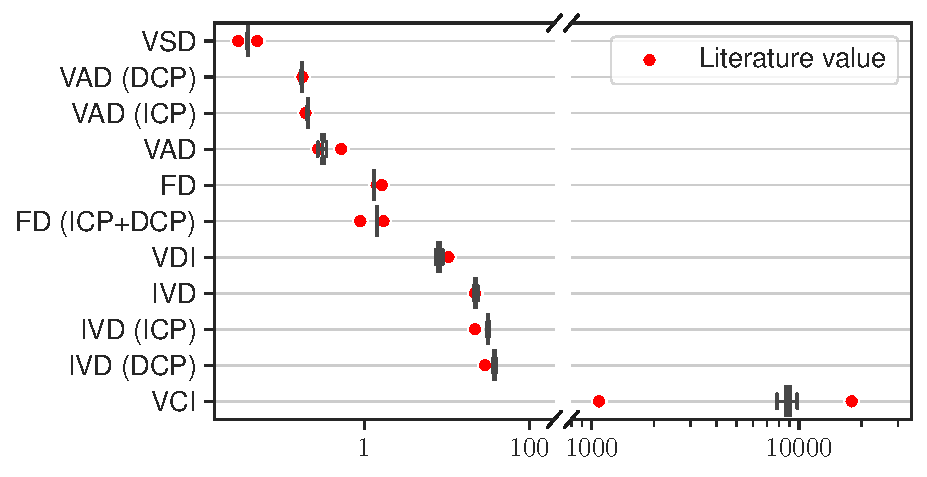
\includegraphics[width=.95\textwidth]{Baseline_metrics}
  \caption{\label{fig:OCTAValidation}Validation of the morphology of virtual vasculatures in the macula against OCTA measurements~\cite{Chu2016,Liu_2021,Ma2021}. Values show the deviation (in \%) from the literature average in healthy eyes. Whiskers extend to the minimum and maximum within \SI{1.5}{} times the inter-quartile range.}  
\end{figure}

The morphology of the macula, within a disk of diameter \SI{4}{\mm} centred at the fovea, is compared to average literature values computed on OCTAs~\cite{Chu2016,Liu_2021,Ma2021} in Figure~\ref{fig:OCTAValidation}.
Except for vascular density, none of those values were used for the development of the model.
Among the remaining metrics, VPI ($\SI{<14}{\percent}$), FD ($\SI{<3}{\percent}$ difference) and IVD ($\SI{<15}{\percent}$ difference) are in good agreement with literature values.

\begin{figure}[ht!]
  \centering
  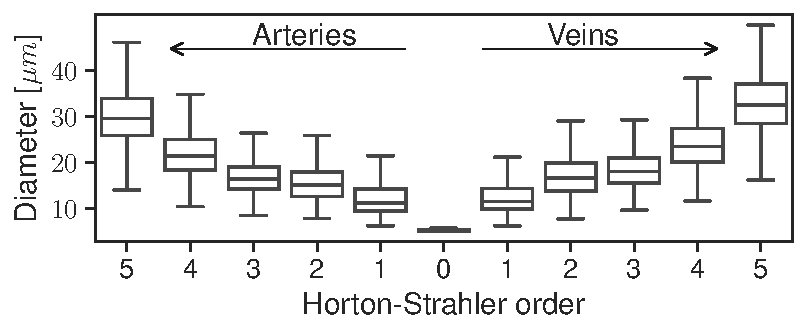
\includegraphics[width=.95\textwidth]{Horton_Strahler_Diameter_Distribution}
  \caption{\label{fig:Horton_Strahler}Box-and-whisker plot of the diameter of virtual vessels for each Horton-Strahler order. On average, close to \SI{5000} vessel segments were analysed for each vasculature. Whiskers extend to the minimum and maximum within \SI{1.5}{} times the inter-quartile range.}  
\end{figure}

Figure~\ref{fig:Horton_Strahler} shows vessel diameters for each stream order in the macula.
The distribution is similar to histological data~\cite{An2020}.
Mean diameters were smaller in the model, but experimental data lay within the ranges of diameters in the model for each order.
The ratio of average arteriole diameter to average venule diameter increased from $\SI{0.91\pm 0.03}{}$
in order 5 vessels to $\SI{0.96\pm0.01}{}$ in order 1 vessels, which is consistent with experimental measurements of $\SI{0.9\pm0.1}{}$~\cite{Goldenberg2013}.  

From the haemodynamics simulations, the mean $\pm$ standard deviation for retinal blood flow, blood velocity in the CRA and macular flow fraction were $\SI[per-mode=symbol]{14.7 \pm 5.6}{\micro\litre\per\minute}$ (range: \SIrange[per-mode=symbol]{3.3}{40.4}{\micro\litre\per\minute}), $\SI[per-mode=symbol]{1.2 \pm 0.2}{\cm\per\second}$ (range: \SIrange[per-mode=symbol]{0.5}{2}{\cm\per\second}) and $\SI{18.4 \pm 3.5}{\percent}$ (ranges: \SIrange{12.0}{27.8}{\percent}).
On average, retinal blood flow in the model was lower compared to experimental studies which reported a mean of \SIrange{30}{40}{\micro\litre\per\minute}~\cite{DoblhoffDier2014,Riva1985}.
Blood velocity in the central retinal artery was also lower in the model compared to the average of \SI{6.3}{\cm\per\second} reported by experimental work~\cite{Dorner2009}.
Blood velocity along the vasculature is compared with experimental studies~\cite{DoblhoffDier2014,Riva1985} in Figure~\ref{fig:Flow-Velocity-dist}A.
Additionally, these studies reported volumetric blood flow rates against diameter. These values are compared with the model's in Figure~\ref{fig:Flow-Velocity-dist}B. 

\begin{figure}[ht!]
  \centering
  \begin{subfigure}[t]{.02\textwidth}
    \scalebox{1}{\adjustbox{valign=T}{\textbf{A}}}
  \end{subfigure}
  \begin{subfigure}[t]{.45\textwidth}
    \scalebox{1}{\adjustbox{valign=T}{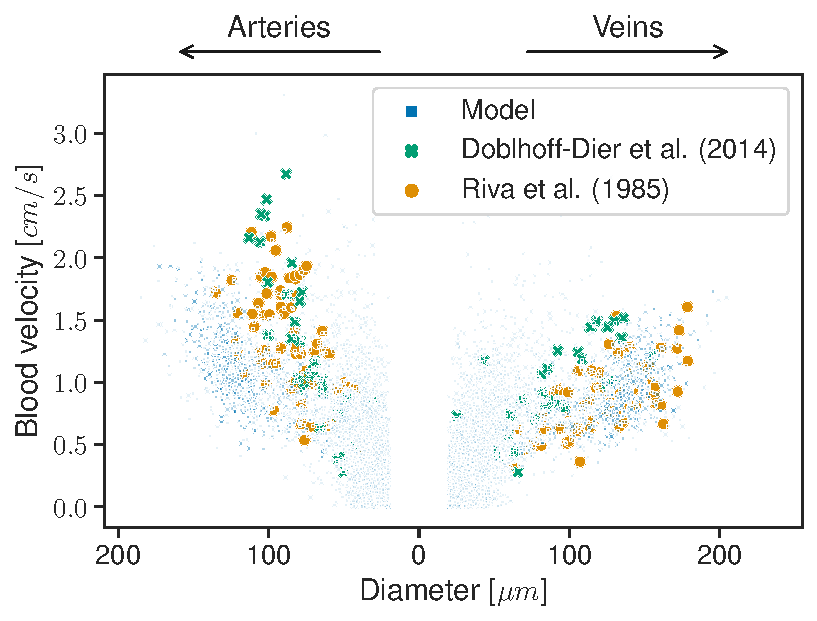
\includegraphics[width=\textwidth]{Velocity_Distribution}}}
  \end{subfigure}
  \hfill
  \begin{subfigure}[t]{.02\textwidth}
    \scalebox{1}{\adjustbox{valign=T}{\textbf{B}}}
  \end{subfigure}
  \begin{subfigure}[t]{.45\textwidth}
    \scalebox{1}{\adjustbox{valign=T}{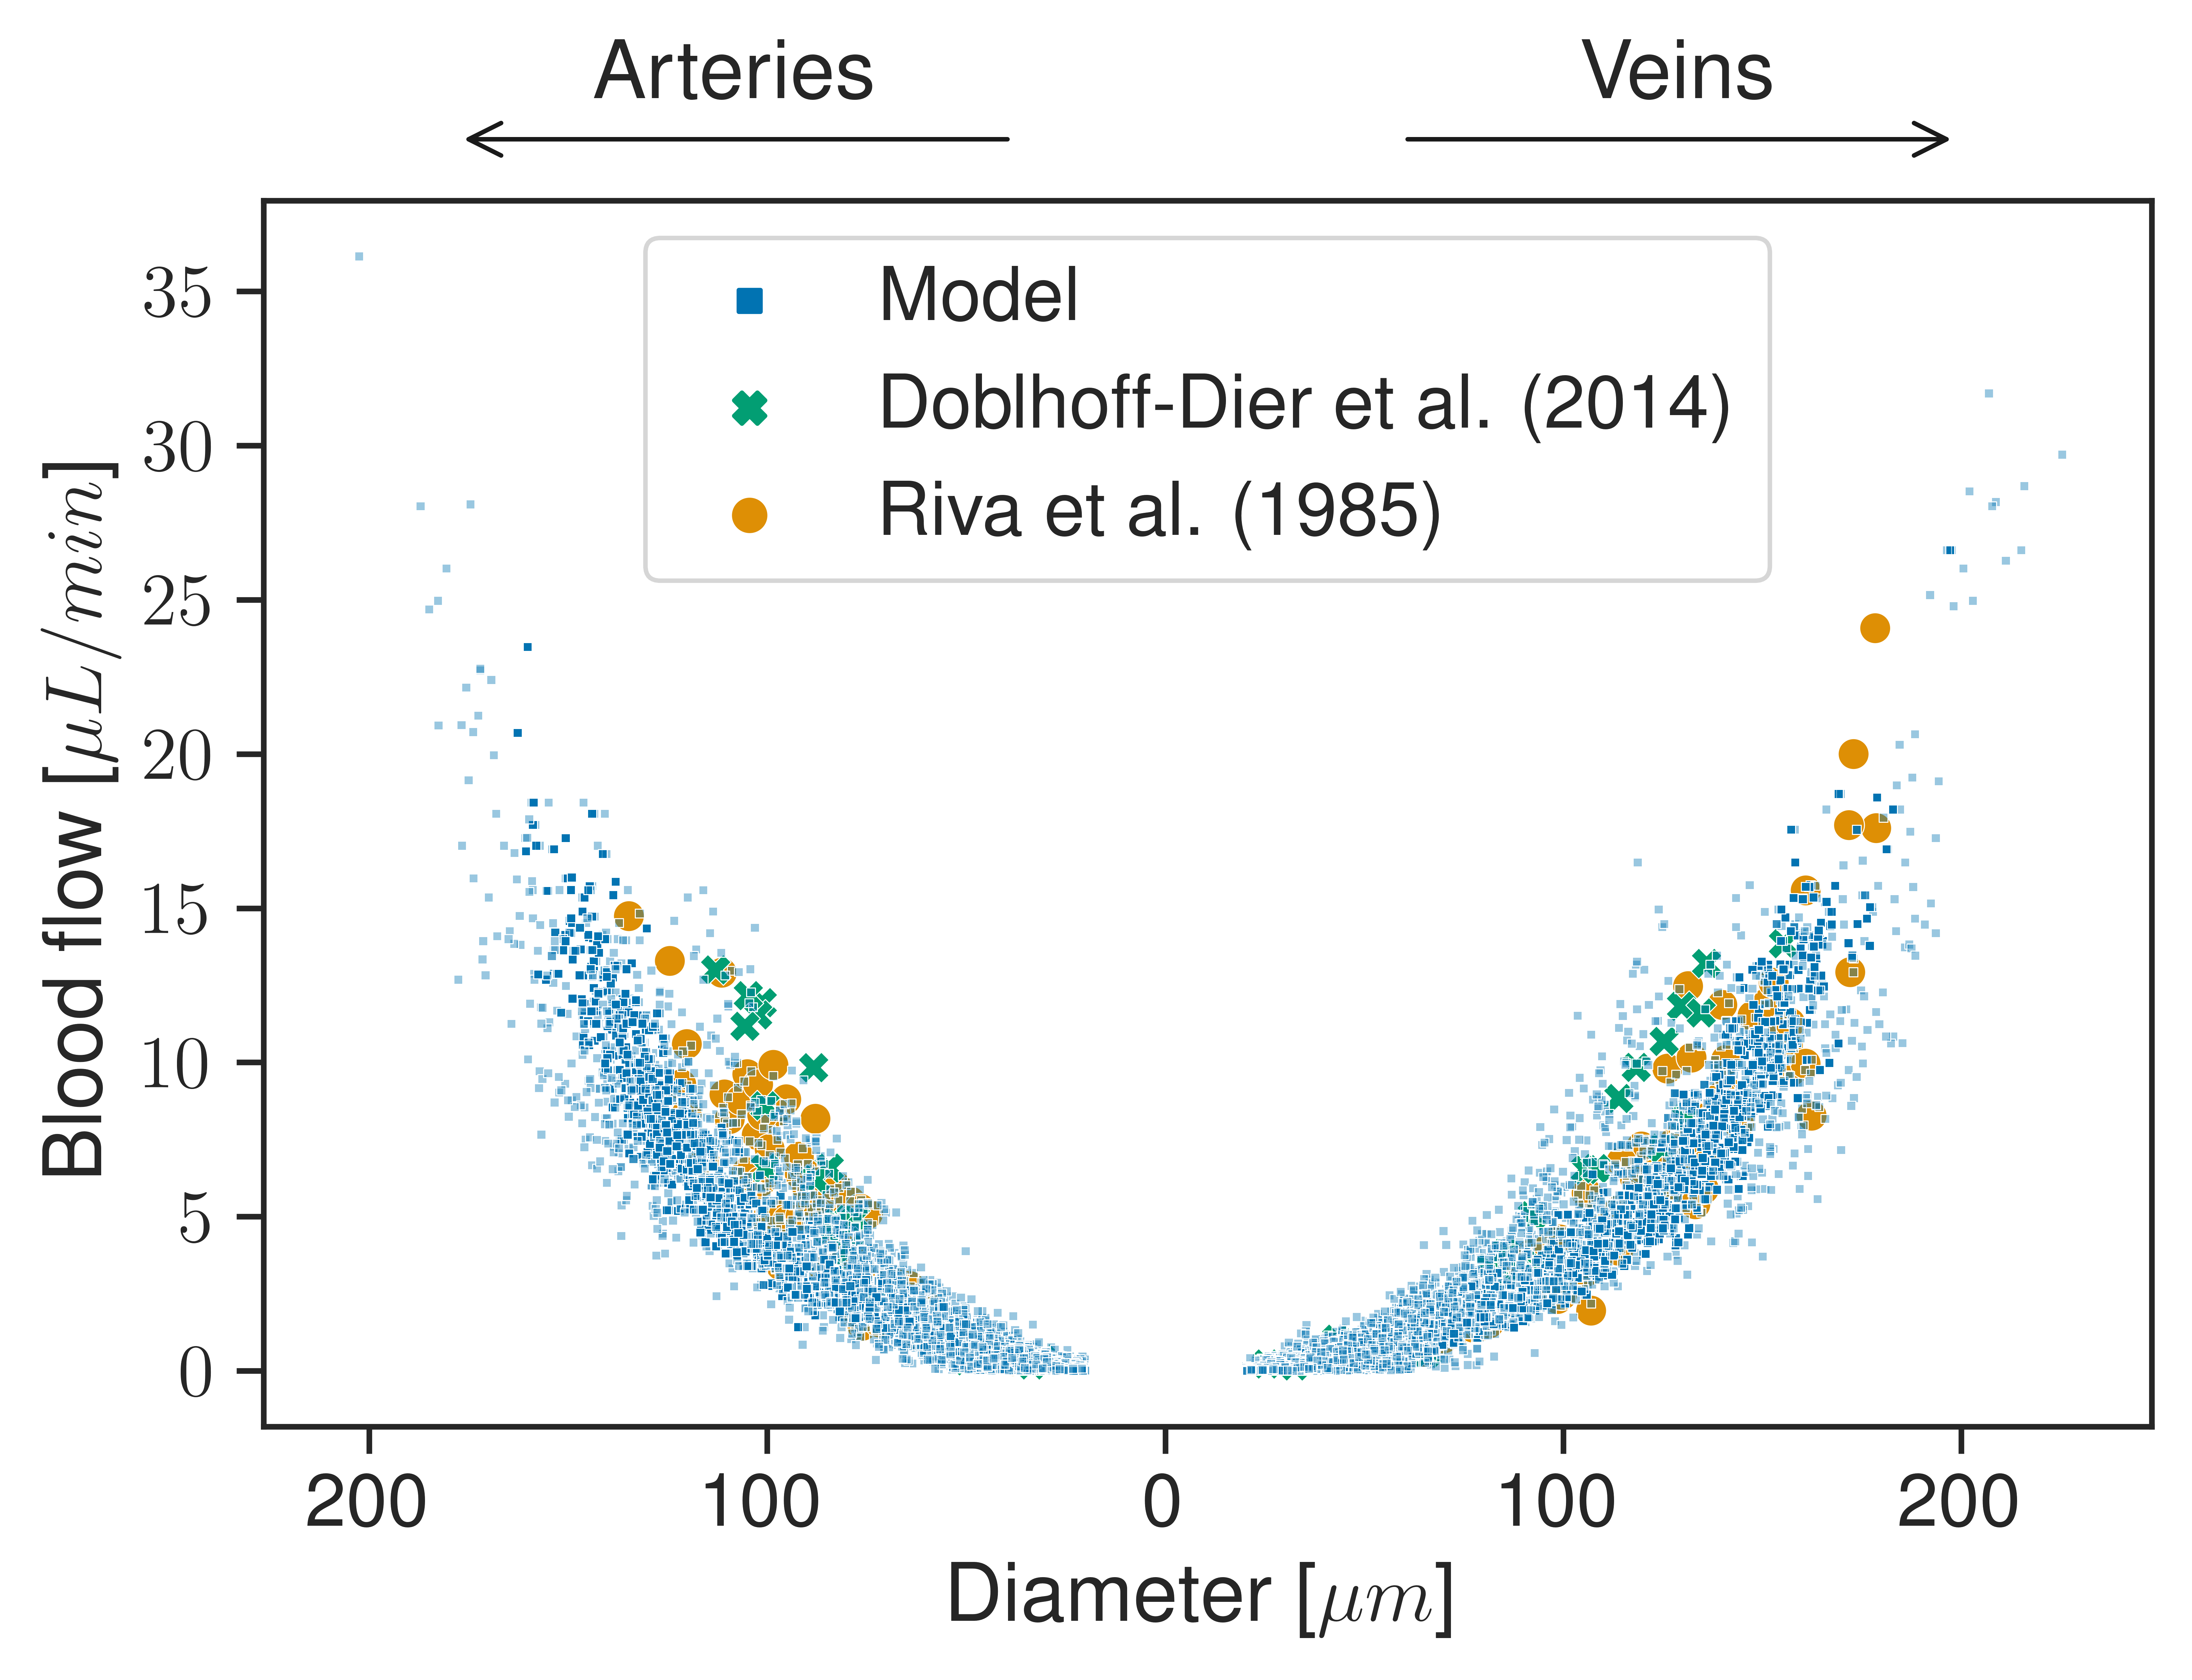
\includegraphics[width=\textwidth]{Flow_Distribution}}}
  \end{subfigure}
  \hfill

  \caption{\label{fig:Flow-Velocity-dist}Blood velocity (\textbf{A}) and volumetric blood flow rate (\textbf{B}) distributions against vessel diameter in the virtual vasculatures compared with two independent experimental studies\cite{DoblhoffDier2014,Riva1985}.}
\end{figure}

\subsection{Four structural variables are strongly linked to retinal function}\label{sec:StructureAndFunction}

We next look to understand how the morphology of the macular vasculature affects the haemodynamics of the retina and of the macula using our model.
Figure~\ref{fig:SpearmanCorrelations} shows the Spearman correlation coefficients for each variables.
Vertical lines show the threshold typically used for a correlation to be considered moderate (dotted lines) and strong (dashed lines).
For the healthy virtual cohort, the model found VAD, VDI, VCI and FD of the SVP to be strong predictors of retinal blood flow, whereas VAD in the ICP and in the combined ICP-DCP complex were found to be moderate predictors.
The correlations with the macular flow fraction were all below \SI{0.25}, indicating weak or no correlations.

\begin{figure}[ht!]
  \centering
  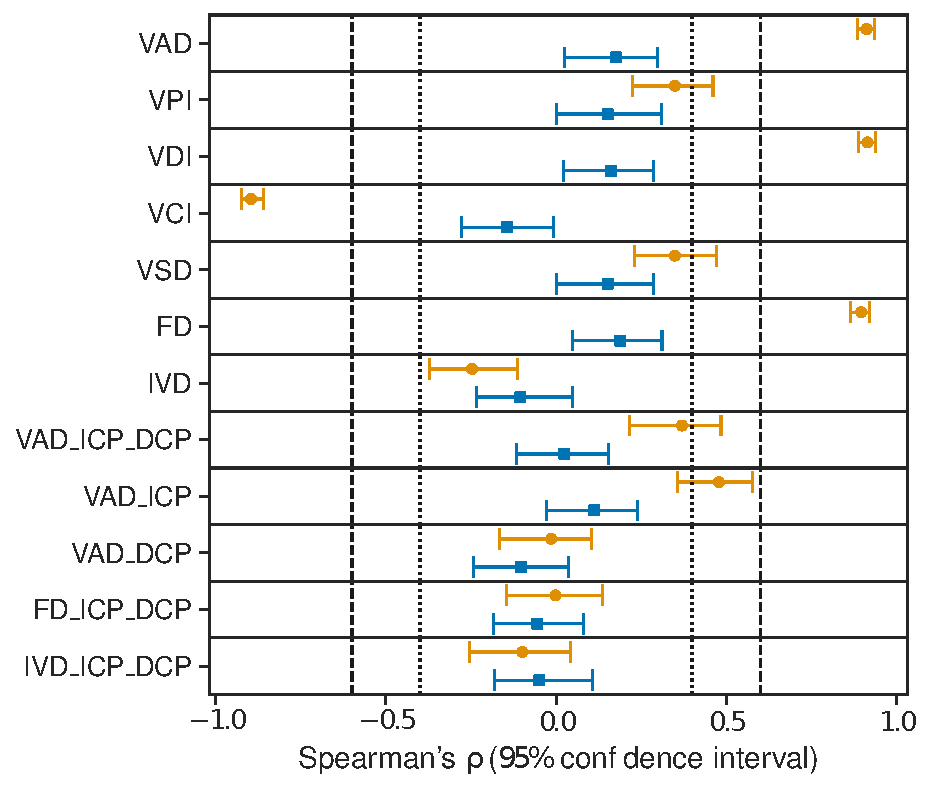
\includegraphics[width=.95\textwidth]{SpearmanCoefficients}
  \caption{\label{fig:SpearmanCorrelations}Spearman correlation coefficients testing for monotonous correlations between morphology and haemodynamics of the macula. Values closer to $1$ or $-1$ indicate stronger correlations. The \SI{95}{\percent} confidence intervals were estimated using bootstrapping.}
\end{figure}

\subsection{Sensitivity analysis and uncertainty quantification}\label{sec:gsaUQ}

\subsubsection{Minimum branching angle dominates structural variability}\label{sec:gsa}

Figure~\ref{fig:gsa}A shows the Sobol indices for \SI{10}{} hyper-parameters, computed with the python library SALib\cite{Iwanaga_2022,Herman_2017} using $\SI{11000}{}$ simulations.
The parameters were sampled uniformly within the ranges presented in Table~\ref{tab:MonteCarloSamplingRanges} using the algorithm by \citet{Saltelli2002}.

For most metrics, all parameters share a similar total order and small first order.
Notably, $\theta_{min}$ stands out as the most influential overall, explaining around \SI{50}{\percent} of the variance in FD and most of the variance in VSD ($S_i=S_{T_i}\approx 1$) by itself.
Other parameters of interest include $N_{seeds}$ for the SVC, $N_{terms}$ for stage 2 and, to a lesser extent, $l_{lim}fr$.
These results indicate that those four parameters are enough to produce a virtual population with inter-population variability, at least in the SVC.

\begin{table}[ht!]
  \centering
  \sisetup{
    range-phrase = \ {;}\ ,
    range-units  = brackets,
    open-bracket = [,
    close-bracket= ],
  }
  \resizebox{\textwidth}{!}{%
    \begin{tabular}{*{10}{l}}
      \toprule
      \begin{tabular}[c]{@{}l@{}}$N_{terms}$\\ stage 2\end{tabular} & \begin{tabular}[c]{@{}l@{}}$N_{terms}$ \\ stage 3\end{tabular} & $l_{lim}f_r$ & $\delta$ & $\eta$ & $\gamma$ & $\nu$ & $\theta_{min}$ & \begin{tabular}[c]{@{}l@{}}Neighborhood\\ factor\end{tabular} & \begin{tabular}[c]{@{}l@{}}$N_{seeds}$ \\ SVC\end{tabular} \\ \midrule
      \SIrange{300}{500}{} & \SIrange{200}{400}{} & \SIrange{0.1}{0.9}{} & \SIrange{0.1}{0.9}{} & \SIrange{0.2}{0.5}{} & \SIrange{2}{3}{} & \SIrange{0}{72}{}  & \SIrange{0}{5}{}  & \SIrange{0}{5}{} & \SIrange{800}{1200}{} \\
      \bottomrule
    \end{tabular}
    }
  \caption{\label{tab:MonteCarloSamplingRanges}Ranges for the hyper-parameters for the computation of Sobol indices.}
\end{table}

\begin{figure}[ht!]
  \centering
  \begin{subfigure}[t]{.03\textwidth}
    \textbf{A}
  \end{subfigure}
  \begin{subfigure}[t]{.95\textwidth}
    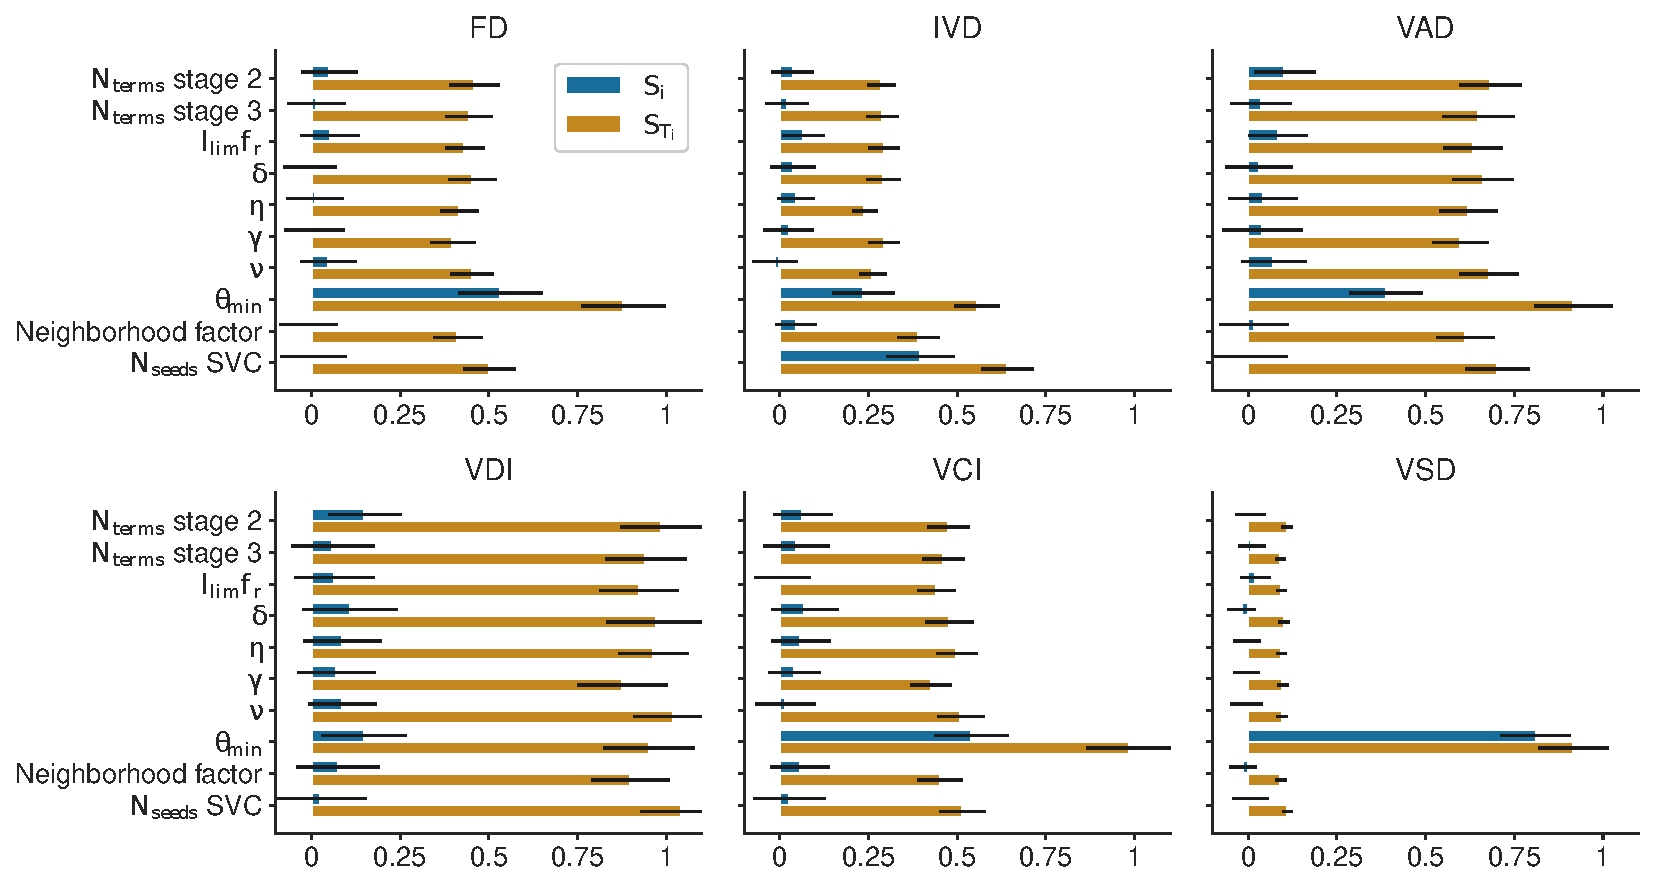
\includegraphics[width=\textwidth, valign=t]{SobolIndices}
  \end{subfigure}
  \\
%  \hfill
  \begin{subfigure}[t]{.03\textwidth}
    \textbf{B}
  \end{subfigure}
  \begin{subfigure}[t]{.95\textwidth}
    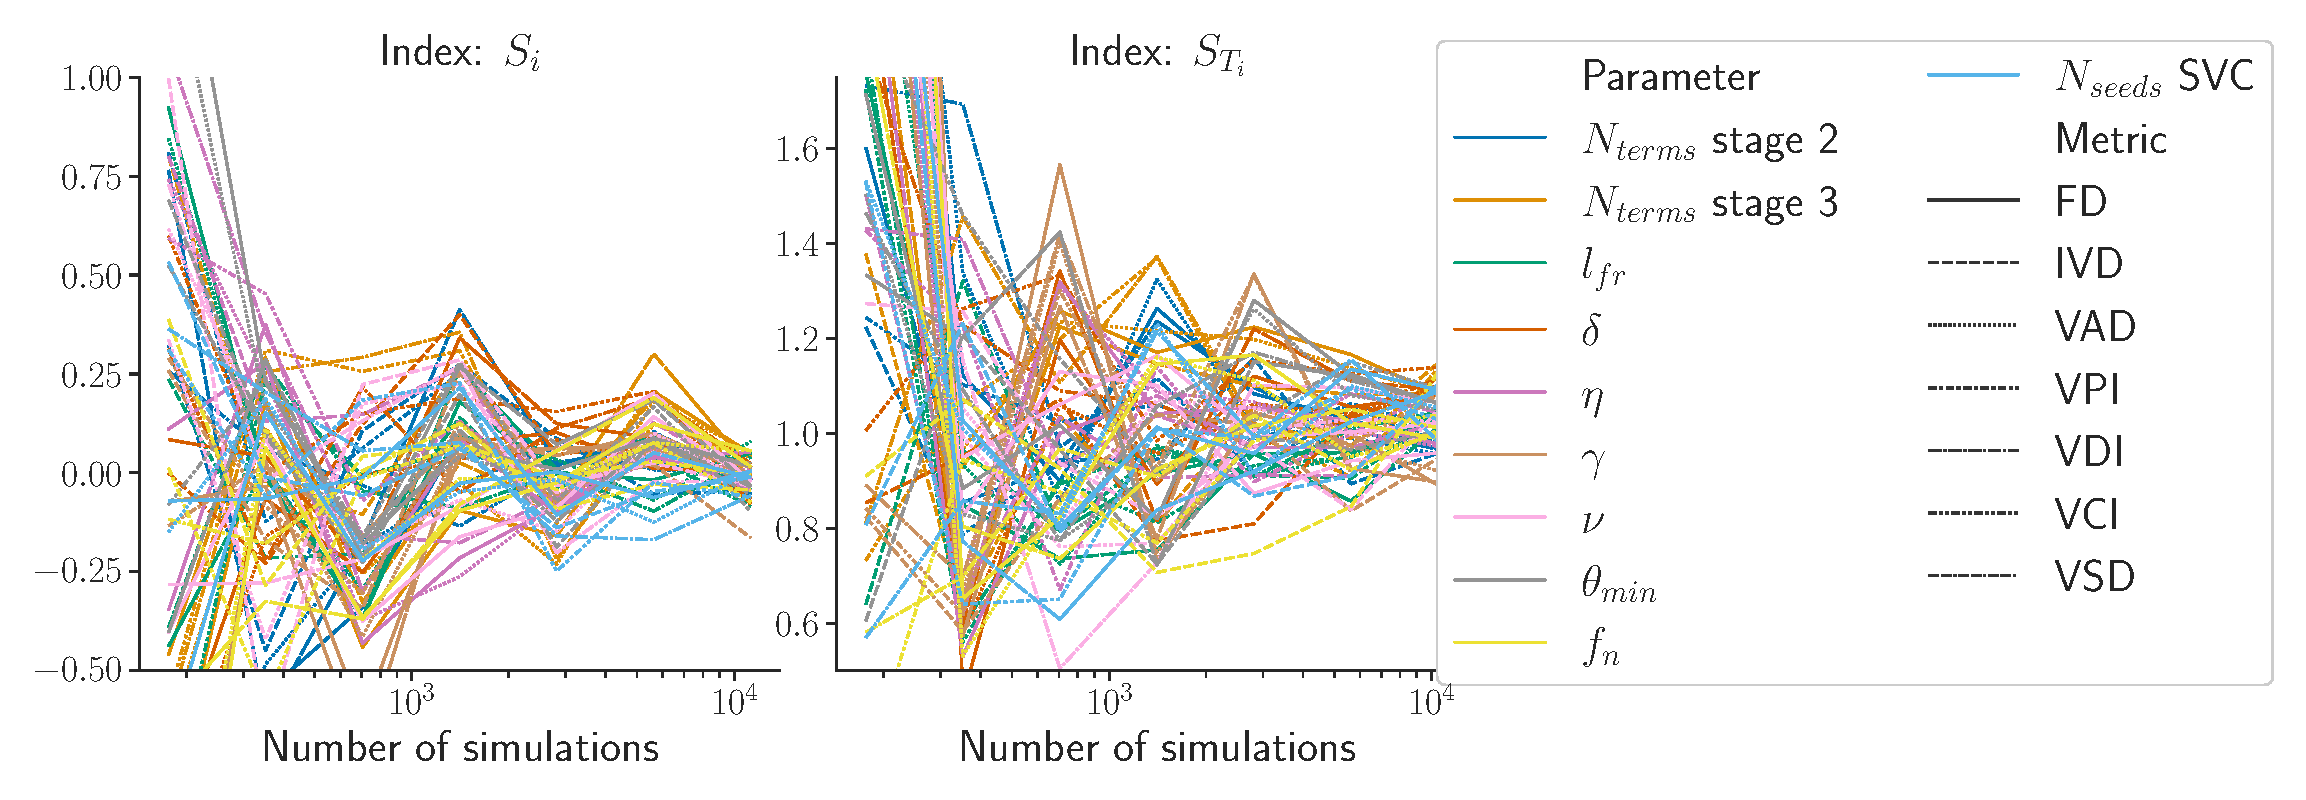
\includegraphics[width=\textwidth, valign=t]{ConvergenceSobolIndices}
  \end{subfigure}
  \caption{Results of the global sensitivity analysis. The bars in (\textbf{A}) show the first order (S1) and total order (ST) Sobol indices for each hyper-parameters of the method with respect to each morphological metrics of the the superficial vascular plexus. 
    The error bars show the \SI{95}{\%} confidence interval for each indices. Convergence of the indices was checked by plotting the indices' values with increasing number of simulations used for their computation (\textbf{B}).}
  \label{fig:gsa}
\end{figure}

\subsubsection{macular flow fraction is independent of OPP}\label{sec:UQ}

The results presented in Section~\ref{sec:results} rely on several hypotheses and parameters which introduce a degree of uncertainty.
Across all scenarios, the mean retinal blood flow varied between \SI{-30.3}{\percent} and \SI{25.2}{\percent} of baseline values whereas macular flow fraction varied between \SI{-17.8}{\percent} and \SI{73.1}{\percent}.
The results for each scenario tested are shown in Table~\ref{tab:sup-UQranges}.
Variation in OPP had almost no effects on macular flow fraction (Pearson's $R^2<10^{-3}$ for all values of $\mathcal R$) but was linearly correlated with retinal blood flow ($R^2>0.81$ for all values of $\mathcal R$).
The coefficients are given for all scenarios in Table~\ref{tab:sup-Pearsonr-UQ}.


\section{Discussion}\label{sec:discussion}

Vascular morphology has been established as a biomarker for the development, progression and prognosis of several retinal diseases~\cite{Balaratnasingam_2023,Yao_2020}, including diabetic retinopathy~\cite{Garg2022,Hein_2023} and age-related macular degeneration~\cite{Told2023,Narnaware_2023}.
Changes in these metrics may indicate impairment to retinal or macular blood flow, which could contribute to the development of the disease. However, quantifying these impairments in a sufficiently large population is challenging with conventional experimental techniques.

The goals of this study were to: 1) develop a method that can generate morphologically and functionally coherent vascular networks of the retina and macula and is applicable to the generation of virtual populations; 2) to quantify the associations between vascular morphology in the macula with haemodynamics quantities in a population of healthy retinae. The method creates a vascular network spanning the superficial layer of the temporal retina, starting from the central retinal artery and ending in the central retinal vein. In the macula, the three capillary layers are modelled. Global sensitivity analysis on the method’s hyper-parameters paves the way for generating specific populations of retinae, based on the distribution of morphological metrics. 

\subsection{Validation}\label{sec:disc-validation}

In Section~\ref{sec:validation}, we validated the models against experimental data.
Figure~\ref{fig:OCTAValidation} showed good agreement with OCTA data for all three layers in terms of VAD, which was used for the development of the method.
Additionally, IVD, FD, VPI and VSD in the SVC were also consistent with literature values~\cite{Chu2016,Ma2021,Liu_2021}.
While VPI values were close to literature values ($\SI{14}{\percent}$ difference), VSD was \SI{35}{\percent} larger in the model.
This could be attributed to an artefact rising from segmentation of the perimeter map in the work by \citet{Chu2016}.
Indeed, the VSD they found is around \SI{16}{\percent} larger than half the VPI value, which is consistent with the discrepancy we found with our model.
Besides, in the virtual populations, the unit is \SI{}{\micro\metre}, whereas in the literature, it is given as $\text{pixel}^{-1}$.
We corrected this by converting the pixels using a \SI{5.7}{\micro\metre\per\text{pixel}} conversion factor~\cite{Spectralis}.
The right conversion factor is difficult to estimate since resolution may vary between OCTA machines, with the curvature of the retina and with the orientation of the vessel with respect to the OCTA's lateral axes. Furthermore, OCTA quantification suffers from many drawbacks: dependence on segmentation methods~\cite{Mehta_2020}, image pre-processing~\cite{Mehta_2019}, noise~\cite{Szpernal2023} and artefacts~\cite{Yao_2020}.
Furthermore, capillaries in the macula are close in diameter to the resolution of standard OCTA~\cite{Chu2016}, which might lead to overestimates of vessel area.
This could also explain the differences, some large, in VCI, VDI, VSD and IVD if we calibrated the hyper-parameters based on a false value of VAD, leading to an unnaturally dense vasculature.

The morphology of the ICP and DCP vasculature was very homogeneous across the generated cohort, as indicated by the narrow inter-quartile ranges in Figure~\ref{fig:OCTAValidation}.
As demonstrated by the sensitivity analysis, this may be resolved by varying $N_{seeds}$, though reasonable bounds need to be defined.

Figure~\ref{fig:Horton_Strahler} showed that the model's distribution of diameters across Horton-Strahler order was similar to experimental data~\cite{An2020}.
However, capillaries were smaller in our model compared to the data.
In their study, \citet{An2020} considered capillaries any vessel with diameter $<\SI{8}{\micro\metre}$, whereas in our model capillaries were assigned a diameter of \SI{5}{\micro\metre} or \SI{10}{\micro\metre} if they are directly connected to an arteriole or venule.
This strategy may be too simplistic to represent the spread of diameters in the vascular bed.
Others have suggested to update the diameter of vessels based on blood pressure from a first haemodynamics simulation~\cite{Linninger2013}.
More in depth analysis of the capillary beds is necessary in order to develop an appropriate strategy.
In the meantime, sensitivity analysis and uncertainty quantification can help improve the reliability of the model.

Figure~\ref{fig:Flow-Velocity-dist} showed that the model's prediction of blood velocity and flow across the vasculature were within range of the experimental data but were both slightly lower in the model predictions\cite{Riva1985,DoblhoffDier2014}.
Similarly, blood flow and velocity in the central retinal artery were both lower in the model compared to experimental data~\cite{DoblhoffDier2014,Riva1985,Dorner2009,Feke_1989}.
As seen in Equations~(\ref{eq:poiseuille}) and~(\ref{eq:resistance}), blood flow and velocity are respectively proportional to the fourth and second power of vessel radius.
Therefore, an increase in radius by a factor of $\sqrt{2}\approx 1.4$ for velocity and $\sqrt[4]{2}\approx 1.18$ for flow would be sufficient to double the model's predictions.
In addition, all parameters in our virtual populations were sampled from independent normal distributions which is likely an incorrect assumption as, e.g., vessel diameter is likely to be correlated with arterial pressure and IOP~\cite{Dziedziak_2022}.
This is exemplified by the three patients with the largest blood flows in our virtual cohort which were between two and three times larger than the average (see Figure~\ref{fig:sup-TRBF}).
These patients shared a similar CRA radius, around \SI{28}{\percent} larger than the cohort's average.
The large difference in retinal blood flow between those three patients was mainly due to differences in OPP.
In experimental studies, the same relation between flow and radius is assumed and blood flow is typically estimated from velocity $v$ and diameter $D$ measurements as $Q=v\pi D^2/4$.
While not as pronounced as for our model, a small measurement error in vessel diameter combined with error in measurement in velocity still results in large deviations from the true blood flow.
Both measurements are challenging and prone to errors~\cite{Leitgeb_2014}.
As discussed by \citet{DoblhoffDier2014}, studies have reported average total retinal blood flow ranging from \SIrange[per-mode=symbol]{30}{80}{\micro\litre\per\minute}\cite{DoblhoffDier2014,Riva1985,Feke_1989}.
Despite the uncertainty in measurements, most studies seem to agree on values in healthy eyes around \SIrange{30}{40}{\micro\litre\per\minute}~\cite{DoblhoffDier2014,Riva1985}.
Despite the difference in total retinal blood flow, Figure~\ref{fig:Flow-Velocity-dist}B shows that the discrepancy with experimental data is reduced as the vessels branch out.

In Section~\ref{sec:UQ}, we quantified the effects of the two parameters of the haemodynamics model on total retinal blood flow and macular flow fraction.
Increasing $\mathcal R$ is similar to gradually closing the connections to/from the vascular compartment.
Therefore, flow is shunted towards the macula and macular flow fraction increases.
Decreasing $\mathcal R$ has an opposite effect, however, the macular flow fraction will eventually reach a plateau when the CRA reaches its maximum capacity in term of blood flow: regardless of the resistance of paths outside the macula, blood will flow through the macula and total retinal blood flow is bounded by physical constraints.
Indeed, in our model, for a given OPP, flow in the CRA is theoretically bounded by the radius and length of the CRA according to Equation~(\ref{eq:poiseuille}).
The same effect explains the non-symmetrical changes in total retinal blood flow as $\mathcal R$ is decreased (see Figure~\ref{fig:sup-UQ-TRBF-MFR-vs-R-OPP}). 

\subsection{Associations between structure and function}\label{sec:disc-results}

Analysis of the \SI{200}{} virtual vasculatures revealed associations between several of the morphological metrics and total retinal blood flow.
In particular, larger VAD, VDI, and FD in the SVC were strongly associated with larger retinal blood flow.
In contrast, larger VCI in the SVC was strongly correlated with smaller retinal blood flow.
Interestingly, VAD in the ICP showed a moderate positive correlation with retinal blood flow.
However, VAD in the DCP and in the combined ICP-DCP complex, as well as FD in the ICP-DCP complex, did not show any significant correlations.
None of the tested metrics were significantly associated with the fraction of flow transiting through the macula.
Uncertainty quantification showed that those results were independent of the haemodynamics model's parameters.
As shown in Figure~\ref{fig:sup-UQ-Coefficients}, varying OPP does not have any effects on the Spearman correlation coefficients.
Increasing the value of $\mathcal R$ shifts the value of the coefficients for macular flow fraction towards the coefficients for total retinal blood flow.
When $\mathcal R$ becomes large, macular flow becomes close to retinal flow, as seen in Figure~\ref{fig:sup-UQ-TRBF-MFR-vs-R-OPP}, therefore increasing the impact of macular morphology on the overall system. 

In Section~\ref{sec:StructureAndFunction}, the correlation coefficients between morphological metrics and haemodynamics were obtained from one-to-one comparisons and therefore do not capture possible interplay between morphological metrics.
Additional analysis is require to better understand which metrics or combination of metrics are strong predictors of blood flow.

\subsection{Developing VPs with a smaller parameter space}\label{sec:disc-gsa}

In Section~\ref{sec:gsaUQ} we presented the results of a global sensitivity analysis of our method's hyper-parameters on the morphology of the vasculature in the SVP.
The results were presented as first and total order Sobol indices for 10 inputs and 6 outputs in Figure~\ref{fig:gsa}A.
These indices were extracted from a large number of simulations in order to ensure convergence, which was reached with around \SI{8000}{} simulations, as seen in Figure~\ref{fig:gsa}B.

The total orders indices were globally similar for all parameters and brought little explanation of the importance of parameters.
Computing second order indices may be necessary to reduce the number of parameters before attempting to generate a different population or to pursue uncertainty quantification.
However, second order indices require larger number of simulations to achieve convergence with Monte-Carlo methods and are therefore expensive to compute~\cite{Saltelli2008}.
In this case, developing a surrogate model (e.g., polynomial chaos expansion) might be required~\cite{Saltelli2008}.
Nonetheless, the first and total order indices suggests that the parameter space can be reduced to as little as four parameters, depending on which morphological metric is deemed more important.

Interestingly, $\theta_{min}$ appeared as the most influential parameter.
In particular, it was the sole parameter influencing VSD.
This results confirms the hypothesis by \cite{Yao_2020} that branch geometry is correlated with VPI, which is twice VSD in Equation~(\ref{eq:OCTAmetrics}).
The associations between structure and haemodynamics should be investigating further, perhaps with spatial metrics which can be compared with OCTA measurements~\cite{Yao_2020}.

\subsection{Limitations}\label{sec:disc-limitations}

Our method had several limitations that should be acknowledged.
We did not model the peripapillary capillary plexus, ignored the curvature of the retina, and assumed a unique inter-plexi connection pattern.
We also assumed that each plexi lay in a two-dimensional plane.
Additionally, as described in Section~\ref{sec:microvasculature}, direct connections between arterioles/venules and capillaries in the SVC were added with a likelihood $\alpha$ which was arbitrarily set to \SI{40}{\percent}.
Similarly, the likelihood of an arteriole or venule to bifurcate to the deeper layers was also arbitrarily set to \SI{30}{\percent}.
The effects of these two values has yet to be assessed.

The effects of uncertainty in measurements (i.e., MAP, IOP, $r_{CRA}$ and $v_{CRA}$) on the generated vasculature remain to be quantified.
The number of hyper-parameters is large and global sensitivity analysis show their effects on vascular metrics to be non-local.
Therefore, directly adapting the method to generate different virtual populations may prove challenging.
Indeed, as stated by \citet{Allen_2016}, efficient generation of virtual populations requires knowledge of plausible ranges for the model parameters and optimising over the set of model parameters.
Reducing the number of parameters to the most influential ones appear necessary and the sensitivity analysis presented in this study is a first step towards this goal.

At this stage, we have not considered the joint distribution of the population parameters such as $r_{CRA}$ and MAP, IOP, $v_{CRA}$.
These are likely to be strongly related and ignoring these associations may create discrepancies in our model's output when compared to experimental data.
However, these joint distributions are not readily available, to the best of our knowledge, but might be inferred from different studies in the future.

The haemodynamics model proposed in this study makes several simplifying assumptions.
In particular, plasma skimming effects, which lead to non-constant haematocrit, and non-Newtonian effects are important aspects of the haemodynamics in the microcirculation which were not incorporated in this model~\cite{Faahraeus1931,Secomb2013}.
Finally, the parameter $\mathcal R$ introduced in this model remains unknown and its value was based on simple computation of the estimated macular blood flow and uncertainty quantification showed that this parameter had a strong effect on the fraction of flow going to the macula.
However, it had limited effect on the total retinal blood flow (at most \SI{30}{\percent} of variation compared to baseline).
In future work, its influence on other haemodynamics measurements should be thoroughly tested.

\section{Conclusion}\label{sec:conclusion}

The method presented in this study provides a framework to study the relationships between structure and function of the retinal vasculature.
It is meant to be adapted to generate virtual populations described by few (4) parameters and a number of quantitative OCTA-based measurements.

In the current study, the model was used to generate a population of healthy eyes and assess the relations between these OCTA measurements and haemodynamics parameters, namely the total retinal blood flow and the fraction of flow transiting in the macula.
Strong association was found between macular morphology and total retinal blood flow and these associations were independent of the input parameters.
The relatively large parameter space may be reduced down to four hyper-parameters for the generation of the vasculature, facilitating the adaptation of the method to generate specific populations.

Further work will focus on generating a different virtual population to assess the whether the model will predict significantly different blood perfusion in diseased maculas.
The model will also be coupled with oxygen delivery models to understand oxygen delivery to the tissue and how it may be affected by microvascular changes.
This methodology, along with the accompanying haemodynamics model, offers an initial step towards gaining insights into the significance of vascular imaging biomarkers in retinal diseases and explore their relationship to no-vascular imaging biomarkers in macular diseases.
Ultimately, this modelling work aims to develop virtual cohorts that can be used in \textit{in silico} clinical trials or to characterise treatment response in retinal diseases.

\bibliography{bibliography}

% \section{Supplementary material}
%\newpage
\supplementarysection

\begin{table}[ht!]
  \centering
\resizebox{\textwidth}{!}{%
\begin{tabular}{@{}llllllllll@{}}
\toprule
 &
   &
     \multicolumn{4}{l}{\begin{tabular}[c]{@{}l@{}}Total retinal blood flow\\ ($\SI{}{\micro\litre\per\minute}$)\end{tabular}} & \multicolumn{4}{l}{macular flow fraction (\%)} \\
  \cmidrule(lr){3-6} \cmidrule(lr){7-10}\\
  R                        & OPP & mean & std & min & max  & mean & std & min  & max  \\
  \cmidrule(r){1-2} \cmidrule(lr){3-6} \cmidrule(l){7-10}
{\SI{5e5}{}}  & 80  & 12.4 & 4.7 & 2.7 & 33.9 & 14.9 & 3.5 & 9.4  & 31.9 \\
 & 100 & 15.5 & 6.0 & 3.4 & 42.9 & 14.9 & 3.4 & 8.5  & 27.1 \\
 & 120 & 18.6 & 7.2 & 4.0 & 51.0 & 14.9 & 3.4 & 8.7  & 28.8 \\
{\SI{1e6}{}} & 80  & 11.8 & 4.5 & 2.6 & 32.4 & 18.1 & 3.6 & 11.8 & 32.7 \\
 & 100 & 14.8 & 5.6 & 3.3 & 40.5 & 18.0 & 3.5 & 10.6 & 31.7 \\
 & 120 & 17.8 & 6.7 & 3.9 & 47.9 & 18.2 & 3.7 & 11.0 & 35.9 \\
\SI{5e6}{} & 80  & 10.2 & 3.7 & 2.5 & 26.4 & 30.7 & 3.8 & 22.6 & 41.7 \\
 & 100 & 12.8 & 4.6 & 3.1 & 32.5 & 30.8 & 3.8 & 21.1 & 44.2 \\
 & 120 & 15.3 & 5.5 & 3.6 & 39.1 & 30.6 & 3.7 & 22.7 & 41.1 \\
  \bottomrule
\end{tabular}%
}
  \caption{\label{tab:sup-UQranges}Results of the 9 scenarios tested for uncertainty quantification.}
\end{table}


\begin{table}[ht!]
\centering
\resizebox{\textwidth}{!}{%
  \begin{tabular}{lllllll}
    \toprule
    Dependent variable    & \multicolumn{3}{l}{$\mathcal R$} & \multicolumn{3}{l}{OPP}\\
    \cmidrule(r){2-4} \cmidrule(l){5-7}\\
    Group                    & OPP = 80 & OPP = 100 & OPP = 120 & R = 500000 & R = 1000000 & R = 5000000 \\
    \cmidrule(r){2-4} \cmidrule(l){5-7}\\
    Total retinal blood flow & 0.88     & 0.89      & 0.87      & 0.98       & 0.98        & 0.95        \\
    macular flow fraction        & 0.89     & 0.89      & 0.88      & 0.00       & 0.00        & 0.00       \\
    \bottomrule
\end{tabular}%
}
\caption{\label{tab:sup-Pearsonr-UQ}Pearson's $R^2$ scores testing linear association between $\mathcal R$ and $OPP$ for the 9 scenarios tested during uncertainty quantification.}
\end{table}

\begin{figure}[ht!]
  \centering
  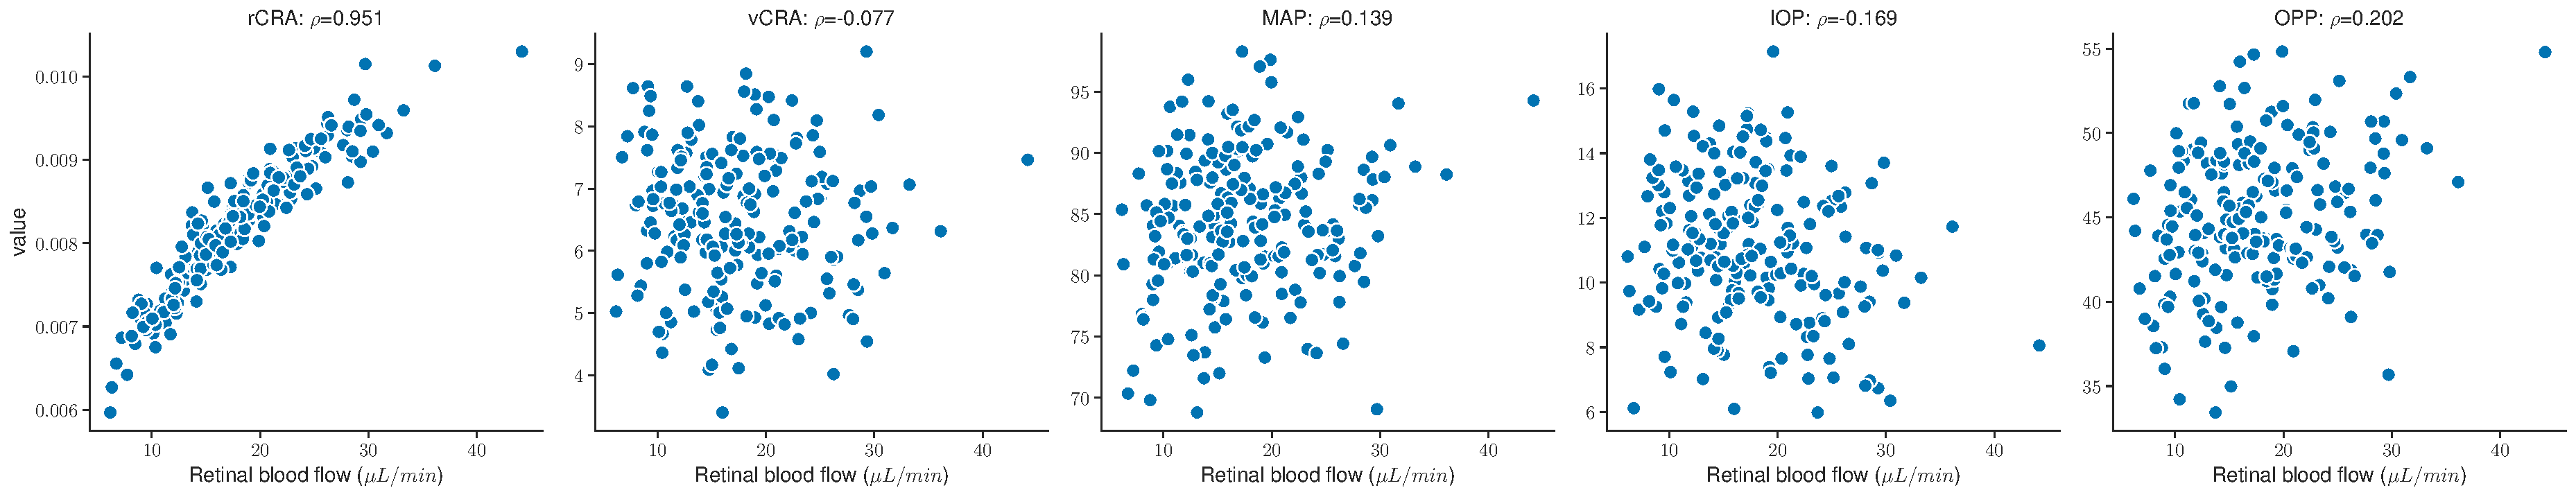
\includegraphics[width=.95\textwidth]{ParametersVP-To-TRBF}
  \caption{Association between retinal blood flow and population parameters. $\rho$ is the Spearman correlation coefficient.}
  \label{fig:sup-TRBF}
\end{figure}

\begin{figure}[ht!]
  \centering
  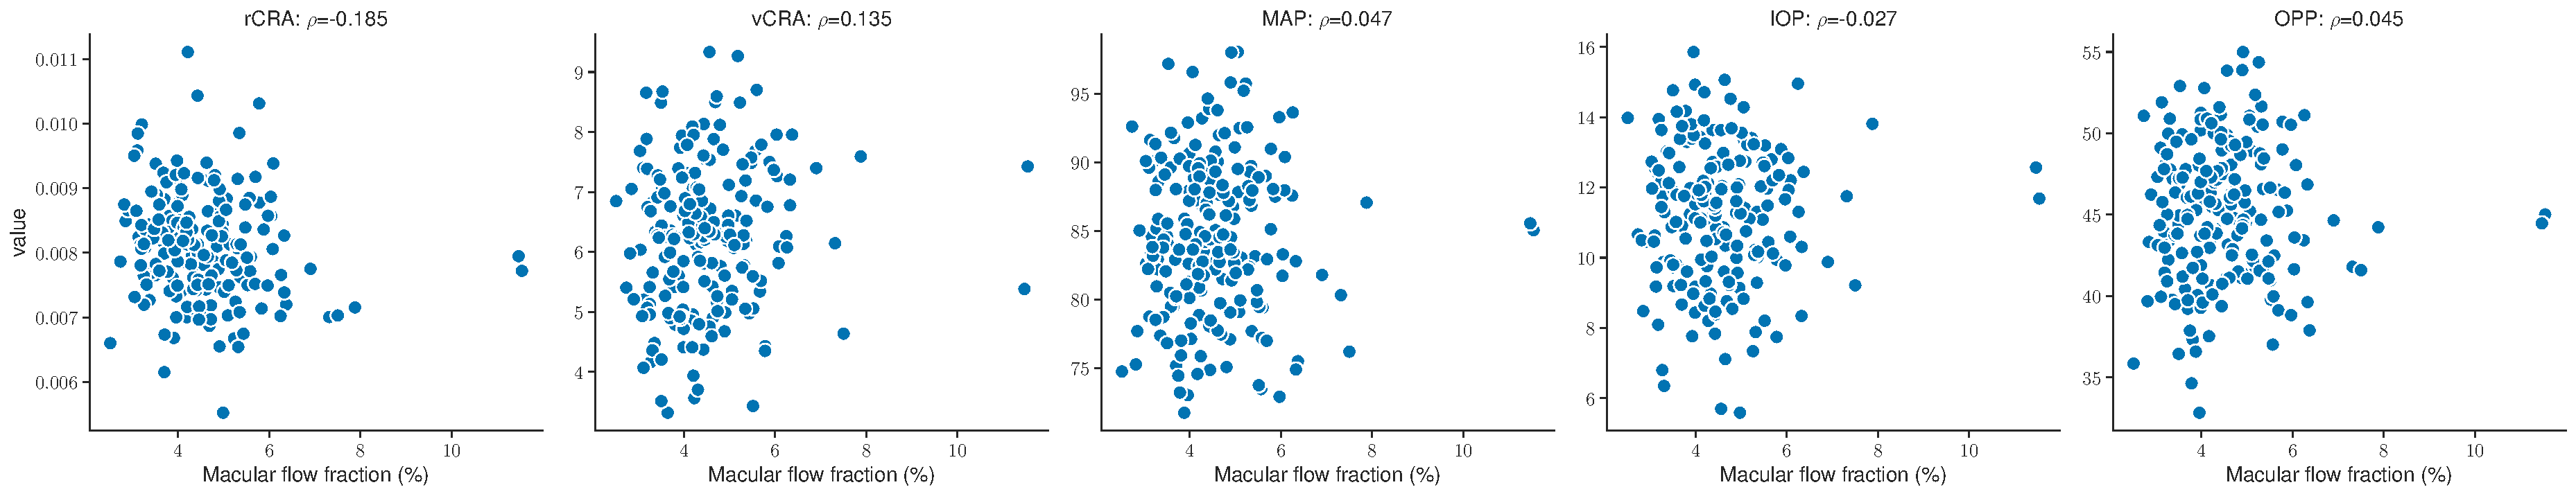
\includegraphics[width=.95\textwidth]{ParametersVP-To-MFR}
  \caption{Association between macular flow fraction and population parameters. $\rho$ is the Spearman correlation coefficient.}
  \label{fig:sup-MFR}
\end{figure}

\begin{figure}[ht!]
  \centering
  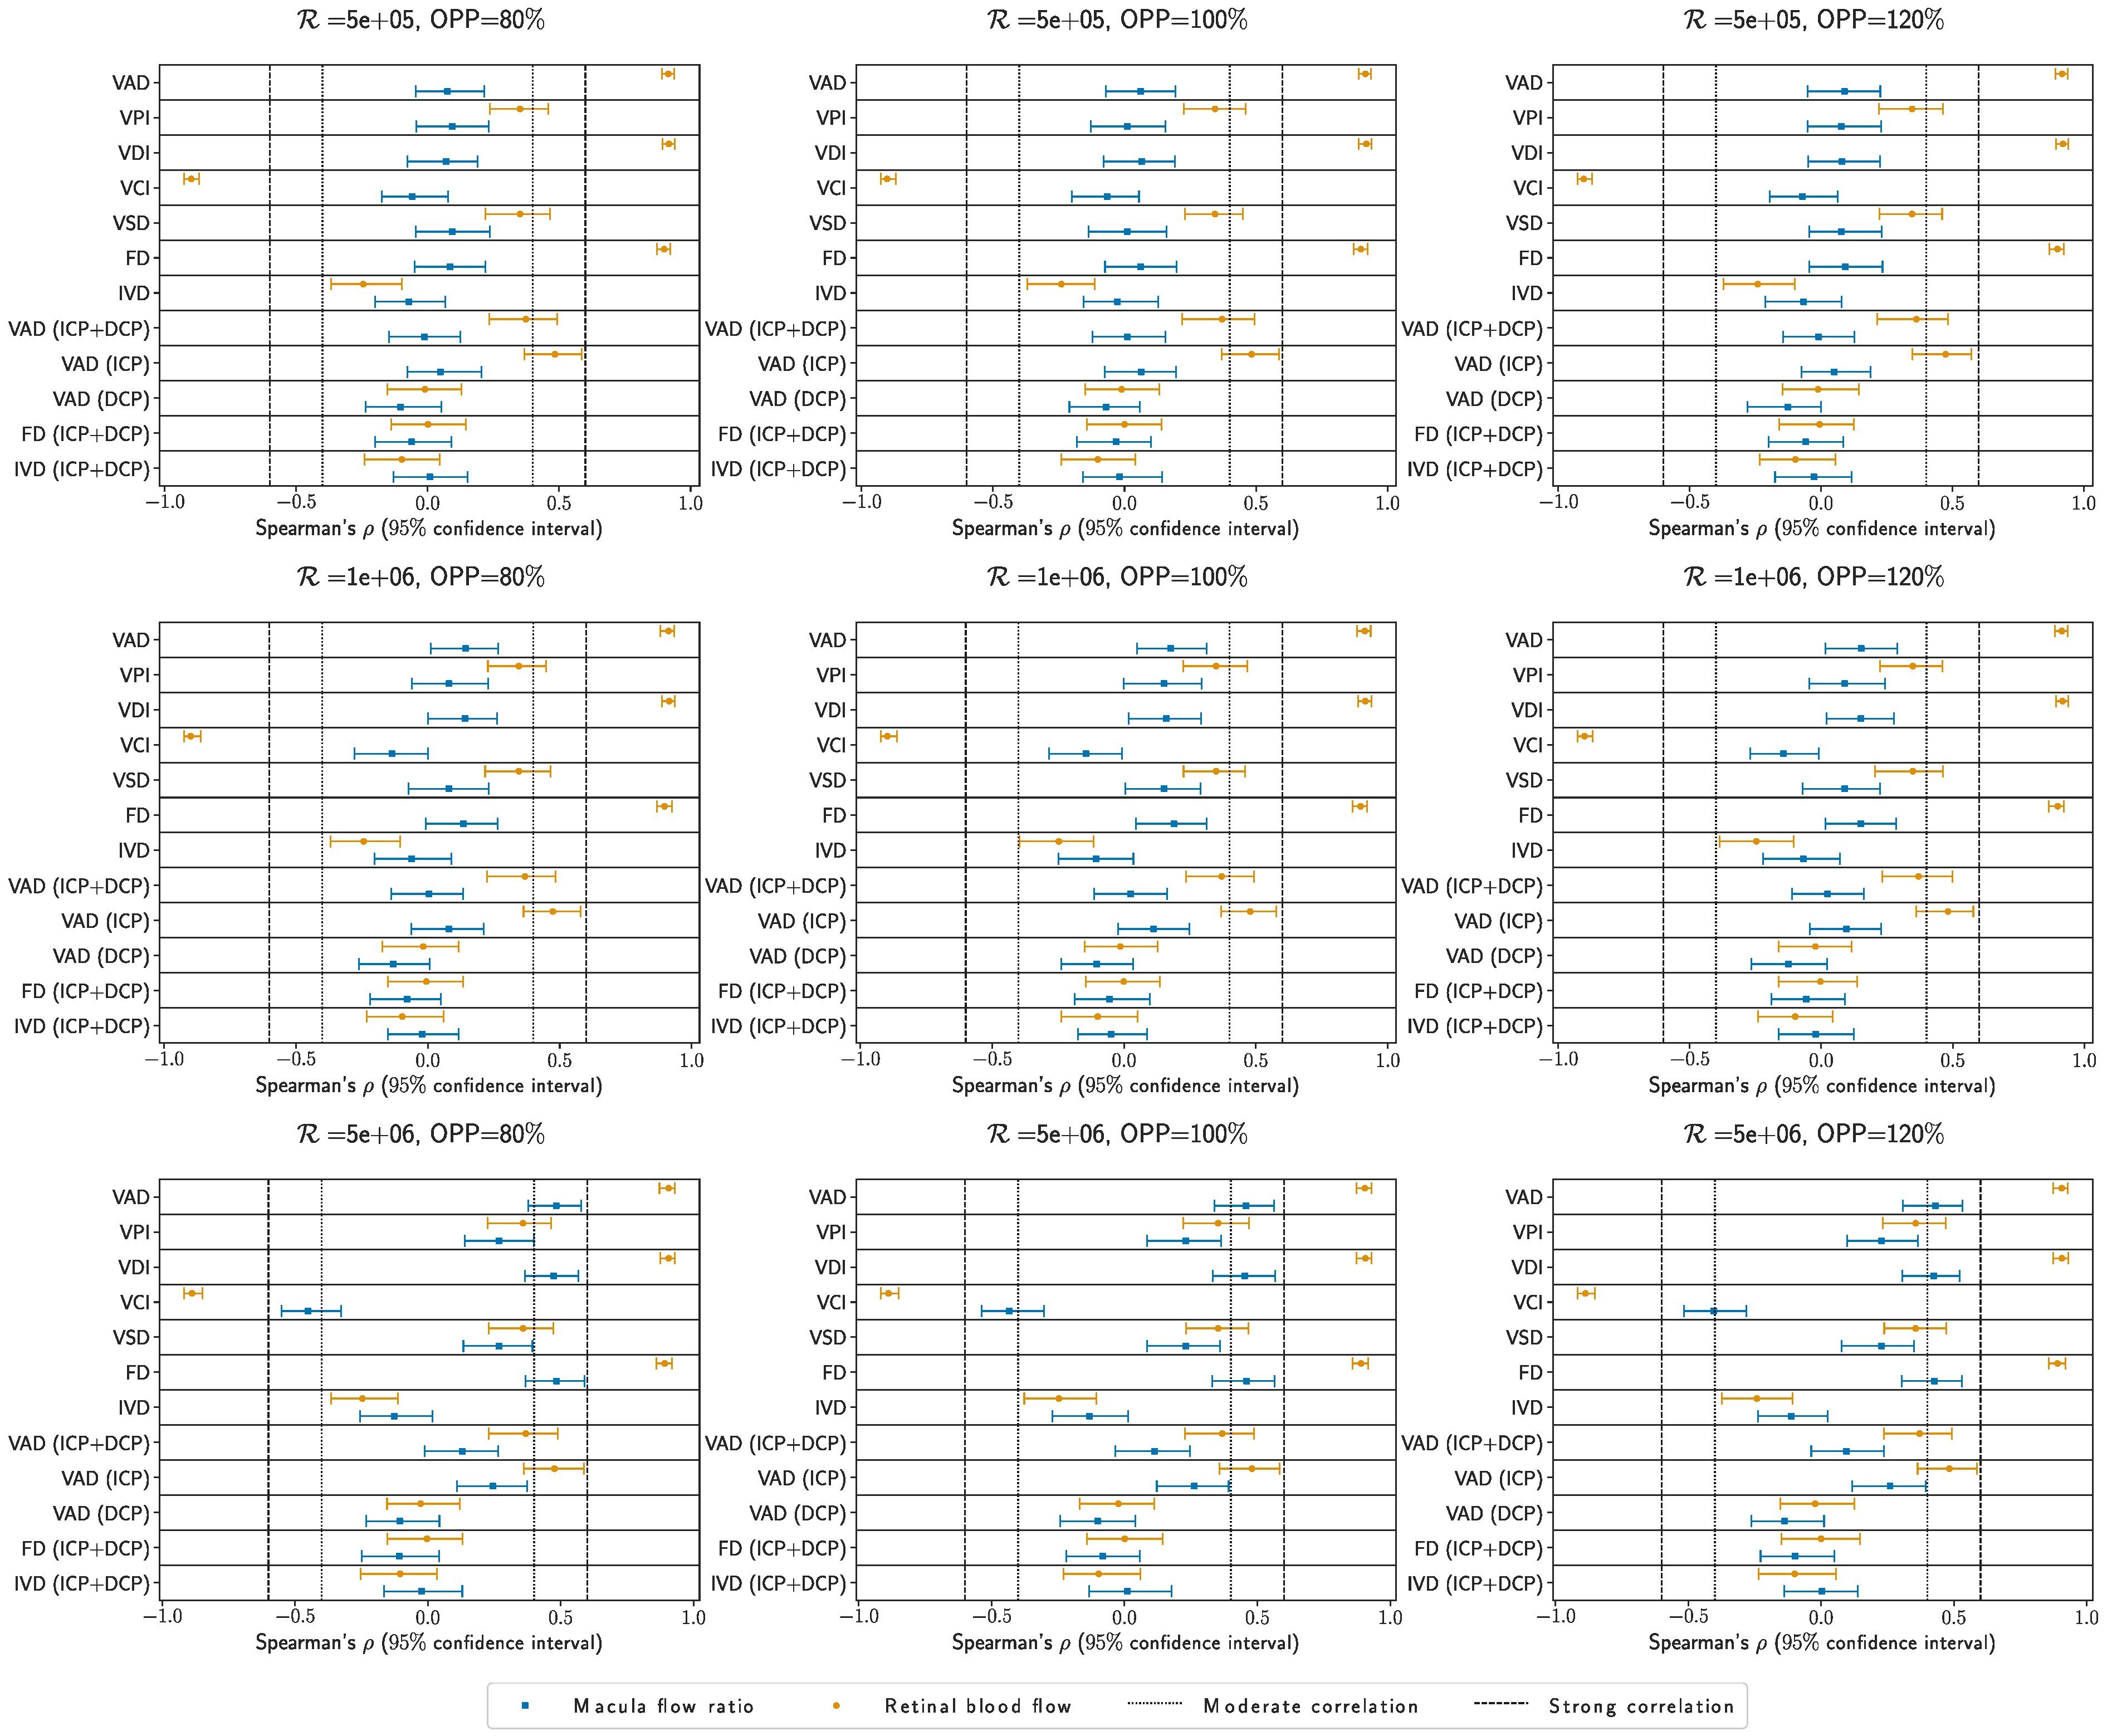
\includegraphics[width=\textwidth]{UQ_SpearmanCoefficients}
  \caption{\label{fig:sup-UQ-Coefficients}Effects of varying OPP and $\mathcal R$ on the associations between structural and haemodynamics outcomes.}
\end{figure}

\begin{figure}[ht!]

  \centering

  \begin{subfigure}[t]{.02\textwidth}
    \scalebox{1}{\adjustbox{valign=T}{\textbf{A}}}
  \end{subfigure}
  \begin{subfigure}[t]{.45\textwidth}
    \scalebox{1}{\adjustbox{valign=T}{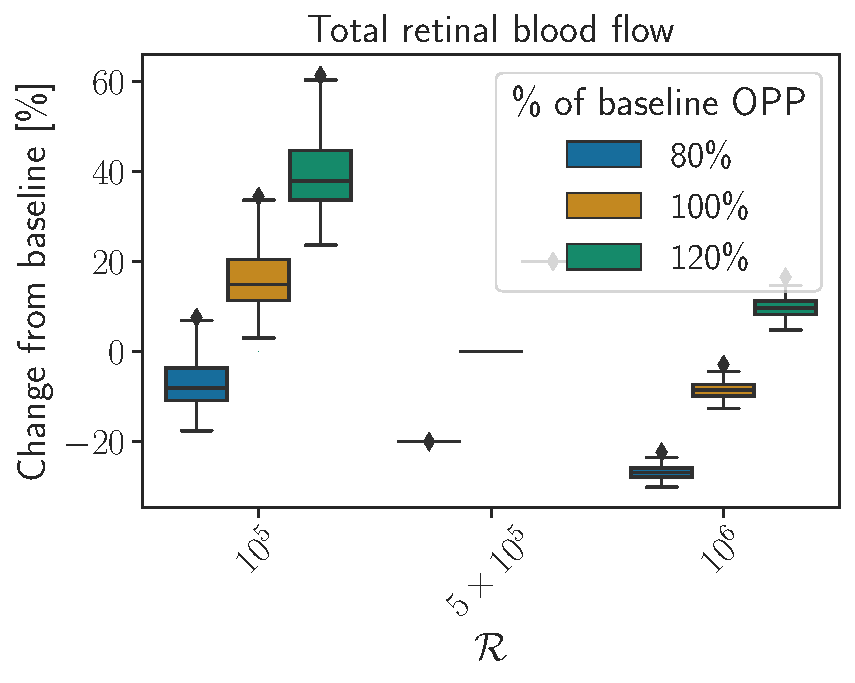
\includegraphics[width=\textwidth]{TRBF_vs_R_OPP}}}
  \end{subfigure}
  \hfill
  \begin{subfigure}[t]{.02\textwidth}
    \scalebox{1}{\adjustbox{valign=T}{\textbf{B}}}
  \end{subfigure}
  \begin{subfigure}[t]{.45\textwidth}
    \scalebox{1}{\adjustbox{valign=T}{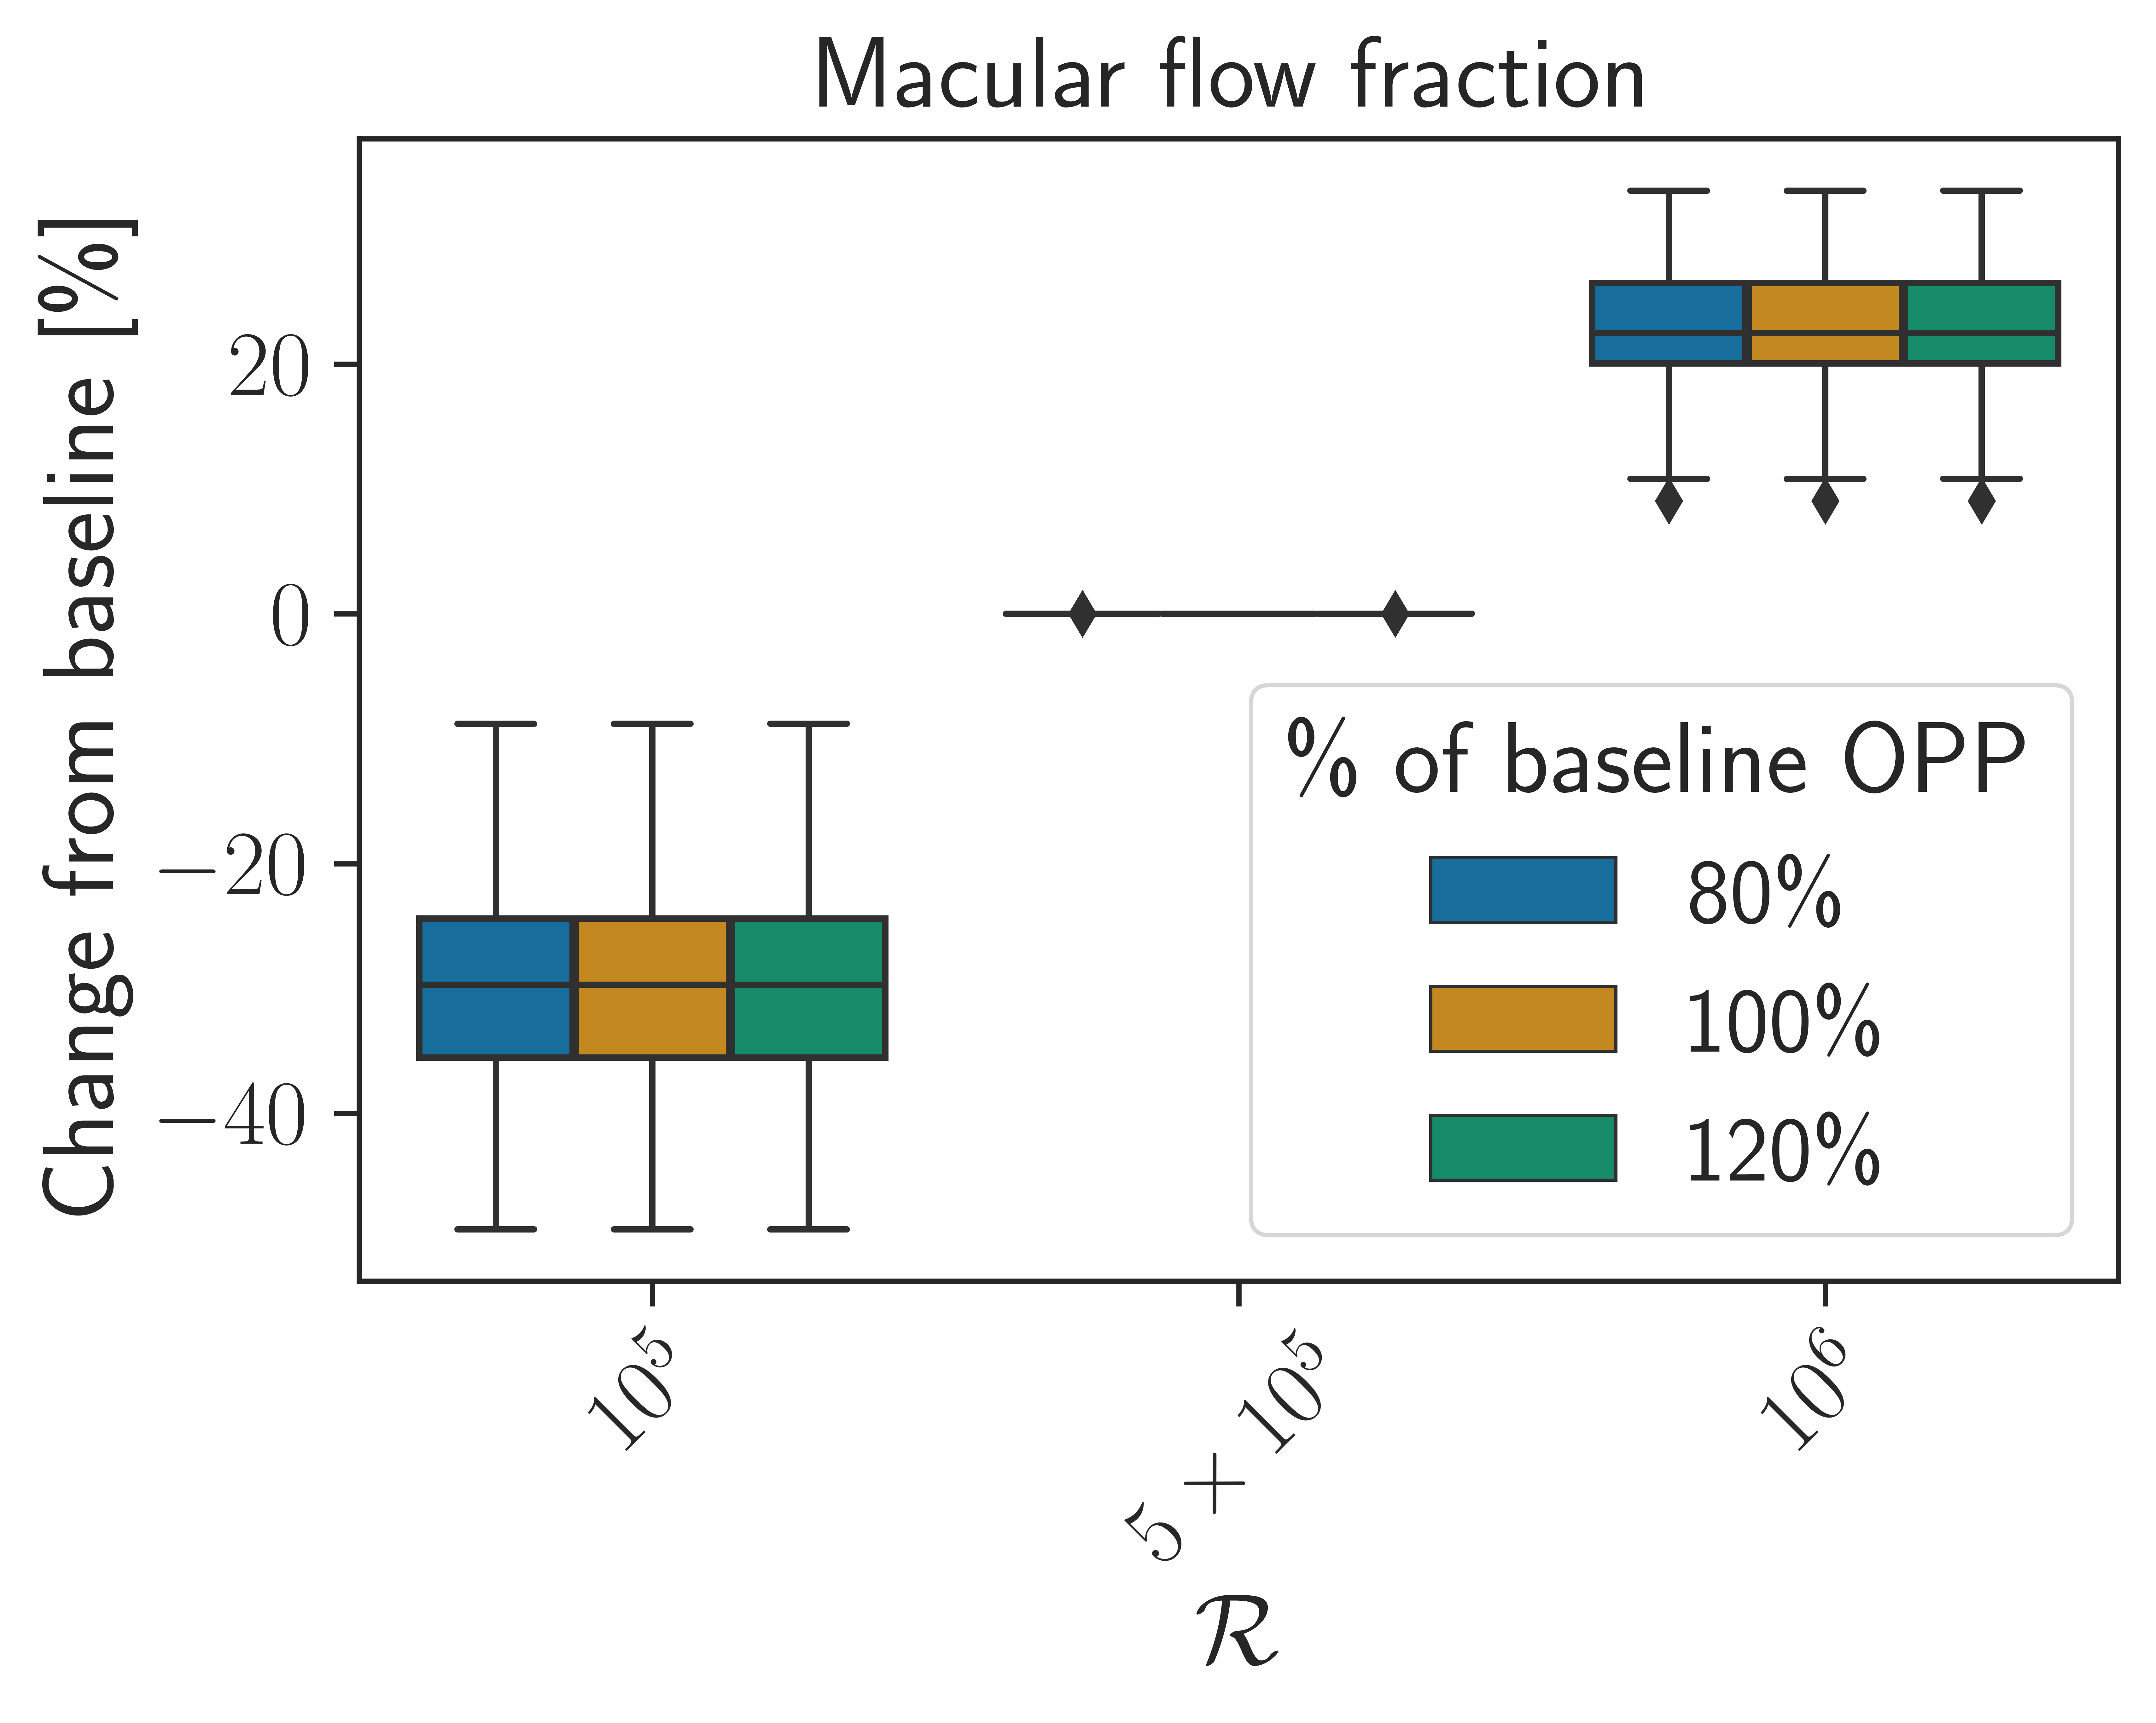
\includegraphics[width=\textwidth]{Maculaflow_vs_R_OPP}}}
  \end{subfigure}
  \hfill
  
  \caption{\label{fig:sup-UQ-TRBF-MFR-vs-R-OPP}Effects of varying OPP and $\mathcal R$ on the haemodynamics outcomes.}
\end{figure}

\end{document}
